
\section{La naturaleza de los datos de serie de tiempo}

El objetivo principal del an\'alisis de series temporales es desarrollar modelos matem\'aticos que proporcionen descripciones plausibles para los datos de la muestra.
\\
Existen dos enfoques metodol\'ogicos b\'asicos para modelar series de tiempo:

	\begin{itemize}
		\item[(i)] El enfoque del dominio del tiempo (Time domain approach)
		\item[(ii)] El enfoque de dominio de frecuencia (Frequency domain approach)
	\end{itemize}

\begin{frame}

El \textbf{enfoque del dominio del tiempo} generalmente est\'a motivado por la presunci\'on de que la correlaci\'on entre los puntos adyacentes en el tiempo de los datos de una serie, se explica mejor en t\'erminos de una dependencia del valor actual en valores pasados. De esta forma, \'este enfoque se centra en modelar alg\'un valor futuro de una serie temporal como una función param\'etrica de los valores actuales y pasados.
\\
En este escenario, por ejemplo, utilizamos modelos de regresiones lineales sobre el valor actual de una serie temporal, utilizando como variables de lado derecho a sus propios valores pasados y los valores pasados de otras series. El seminal trabajo de Box y Jenkins y sus modelos autoregresivos (ARIMA), se encuentran en esta l\'\i{}nea, ver \cite{BoxJenkins}.

\end{frame}

\begin{frame}

Por otro lado, \textbf{el enfoque de dominio de frecuencia} asume que las caracter\'\i{}sticas principales de inter\'es en el an\'alisis de las series de tiempo se relacionan con variaciones sinusoidales peri\'odicas o sistem\'aticas que se encuentran naturalmente en la mayor\'\i{}a de los datos.
\\
Estas variaciones peri\'odicas a menudo son causadas por fen\'omenos biol\'ogicos, f\'\i{}sicos o ambientales de inter\'es. El estudio de la periodicidad se extiende a la econom\'\i{}a y las ciencias sociales, donde uno puede estar interesado en las periodicidades anuales en series como el desempleo mensual o las tasas mensuales de natalidad.
\\
En el an\'alisis espectral, la partici\'on de los diversos tipos de variaci\'on peri\'odica en una serie temporal se lleva a cabo evaluando separadamente la varianza asociada con cada tipo de periodicidad.

\end{frame}
\pagebreak
%\begin{frame}
\subsection{Ejemplo 1: Cambio climático}Nuestro primer ejemplo de serie de tiempo es la temperatura de la tierra. Observamos una aparente tendencia ascendente en la serie durante la \'ultima parte del siglo XX, la que se ha utilizado como argumento para la hip\'otesis del calentamiento global. N\'otese tambi\'en la tendencia ascendente y bastante pronunciada alrededor de 1970. La cuesti\'on de inter\'es para los defensores del calentamiento global y los oponentes es si la tendencia general es natural, o si por el contrario es causada por el ser humano.

\begin{figure}[H]{}
	\centering
	\textbf{Ejemplo 1: Cambio climático}\par\medskip
	\fcolorbox{green}{blue}{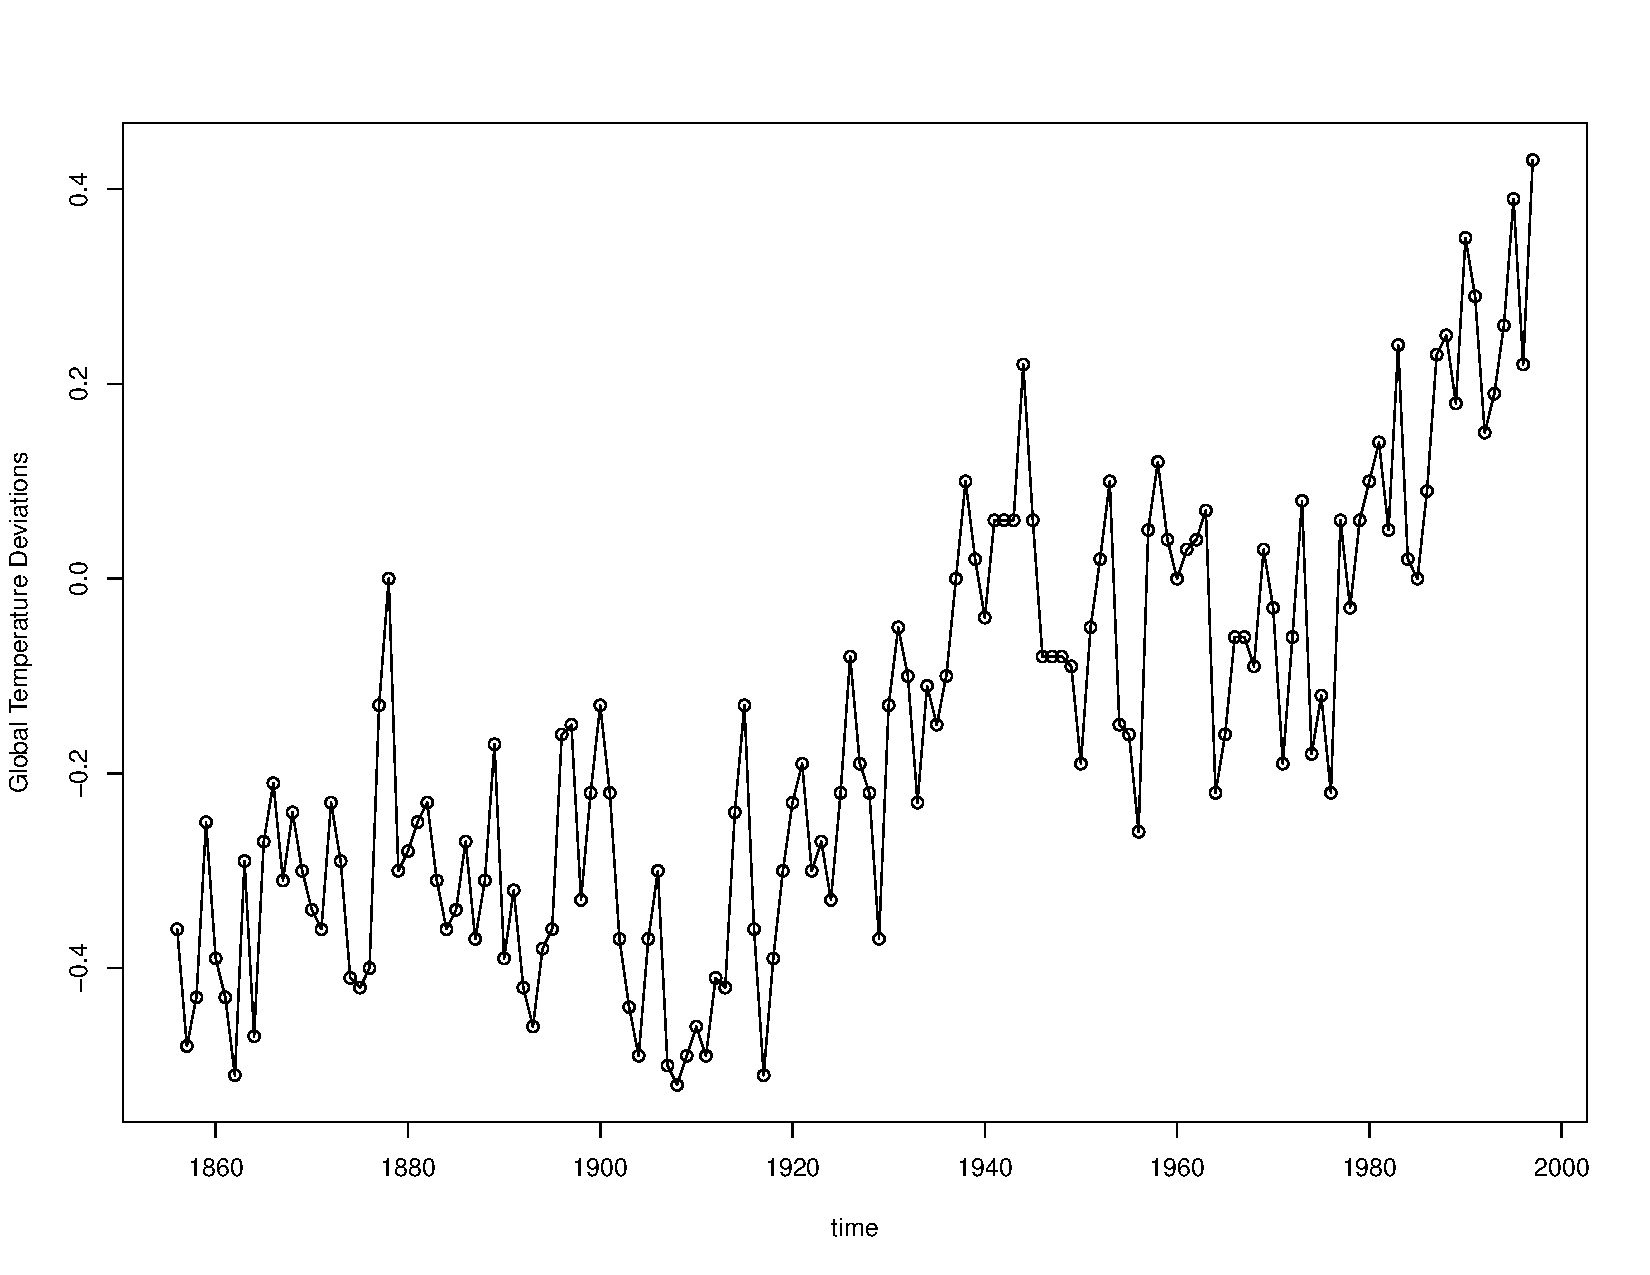
\includegraphics[width=\linewidth]{gtemp.pdf}}
	\caption{Cambio clim\'atico: mediciones de temperatura desde 1860}\label{figura1}
\end{figure}
%\end{frame}

%\centering
\lstset{caption=Código R para ejemplo del cambio climático,framexleftmargin=5mm, frame=shadowbox, rulesepcolor=\color{green}}
\pagebreak
\begin{lstlisting}[title={‘Código R  para ejemplo del cambio climático.’},basicstyle=\ttfamily]{}
# Set the working directory
setwd("/Users/Desktop/Econometrics/Clase 1.- TSE")
# Limpiar_variables
rm(list=ls())

install.packages("tidyverse")
install.packages("dplyr")
install.packages("tseries")

mydata<-read.csv ("gtemp.csv")
plot(mydata, type="o", ylab="Global Temperature Deviations")
\end{lstlisting}

%---------------------Slide 9 --------------------------
%\begin{frame}
\subsection{Ejemplo 2: Series temporales financieras}
%\frametitle{Ejemplo 2: Series temporales financieras}
En finanzas siempre es preferible trabajar con el retorno (returns) de los activos, en vez de usar directamente el precio de los activos. Existen dos maneras de convertir el precio en retornos:
\begin{equation*}
R_t = \frac{p_t - p_{t-1}}{p_{t-1}} *100%
\end{equation*}
\\
\begin{equation*}
R_t = ln\left(\frac{p_t}{p_{t-1}}\right)*100%
\end{equation*}
where, $R_t$ denota el retorno al tiempo $t$, $p_t$ denota el precio del activo al tiempo $t$, y $ln$ denota el logaritmo natural. En esta formulaci\'on ignoramos los dividendos, o asumimos que las series de precios ya han sido ajustadas por ellos.

%\end{frame}
%---------------------Slide 10 --------------------------
%\begin{frame}
%\frametitle{Ejemplo 2: Series temporales financieras}
Los log-returns tienen la deseable propiedad de poder ser interpretados como rendimientos continuamente compuestos. Adem\'as, ellos pueden ser simplemente sumados, de forma de obtener retornos con respecto a per\'\i{}odos m\'as largos:
\begin{center}
	$r_1 = ln \frac{p_1}{p_0} = ln p_1 - ln p_0$\\
	$r_2 = ln \frac{p2}{p_1} = ln p_2 - ln p_1$\\
	$r_3 = ln \frac{p3}{p_2} = ln p_3 - ln p_2$\\
	$r_4 = ln \frac{p4}{p_3} = ln p_4 - ln p_3$\\
	$r_5 = ln \frac{p5}{p_4} = ln p_5 - ln p_4$\\	
	\vspace{5mm}	     			      
	$r_1+r_2+r_3+r_4+r_5=ln p_5 - ln p_0    =  ln \frac{p_5}{p_0}$\\
\end{center}
%\end{frame}
%---------------------------------------------------------
%\begin{frame}
%\frametitle{Ejemplo 2: Series temporales financieras}
\subsubsection{Ejemplo 2: Series temporales financieras}
Como segundo ejemplo calcularemos los retornos de la Bolsa de Nueva York, \'\i{}ndice "S$\&$P 500", extrayendo data diaria desde el a\~no 2000, del sitio: https://finance.yahoo.com/\\

%\only<1|handout:1>{
	%\begin{exampleblock}{C\'odigo en R}
\lstset{caption=Código R precio de la Bolsa de Nueva York,framexleftmargin=5mm, frame=shadowbox, rulesepcolor=\color{green}}
\begin{lstlisting}[title={‘Código R precio de la Bolsa de Nueva York.’},basicstyle=\ttfamily]{}
mydata2<-read.csv("sp.csv")
precio<-mydata2$"Adj.Close"
plot.ts(precio, type="o", ylab="Precio Bolsa de Nueva York")
lnprecio <- log10(precio)
Dlnprecio <- diff(lnprecio,1)
plot.ts(Dlnprecio, type="o", ylab="Retorno Bolsa de Nueva York")
summary (lnprecio)
summary (Dlnprecio)
\end{lstlisting}

%\end{exampleblock}
%}
%\end{frame}
%---------------------------------------------------------
%---------------------Slide 12 --------------------------
%\begin{frame}
%\frametitle{Ejemplo 2: Series temporales financieras}
%\textbf{Indice Bolsa de Nueva York}
%\end{frame}
\begin{figure}[H]{}
\centering
\textbf{Ejemplo 2: Series temporales financieras}\par\medskip
\fcolorbox{green}{blue}{
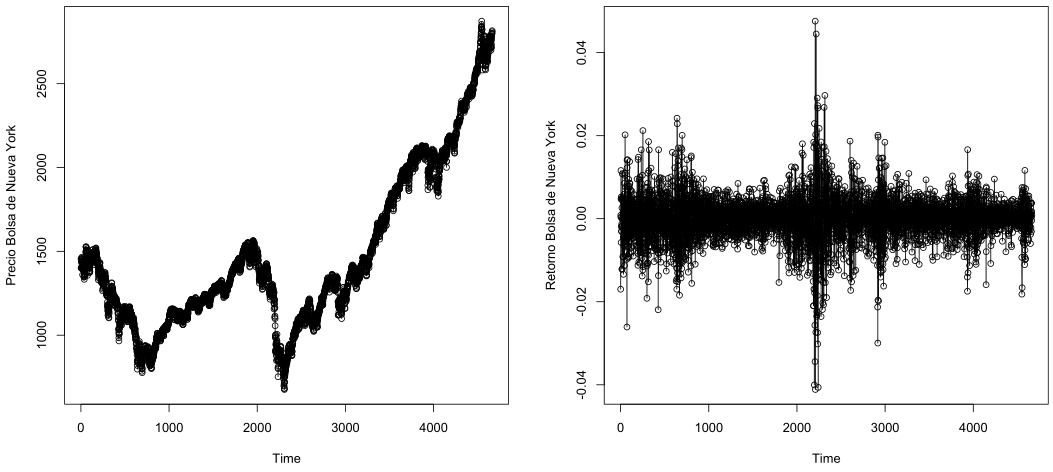
\includegraphics[width=\linewidth]{bolsaNYD12.png}}
\caption{Indice Bolsa de Nueva York. Izquierda: precios reales SP500. Derecha: retornos SP500.}\label{figura2}
\end{figure}

%---------------------------------------------------------
%---------------------Slide 13 --------------------------
%\begin{frame}
%\frametitle{Ejemplo 2: Series temporales financieras}
Los precios al parecer no son normales, aparentemente son log-normales.\\
\begin{figure}[H]
	\centering
	\textbf{Ejemplo 2: Histograma de los Precios}\par\medskip
	\fcolorbox{green}{blue}{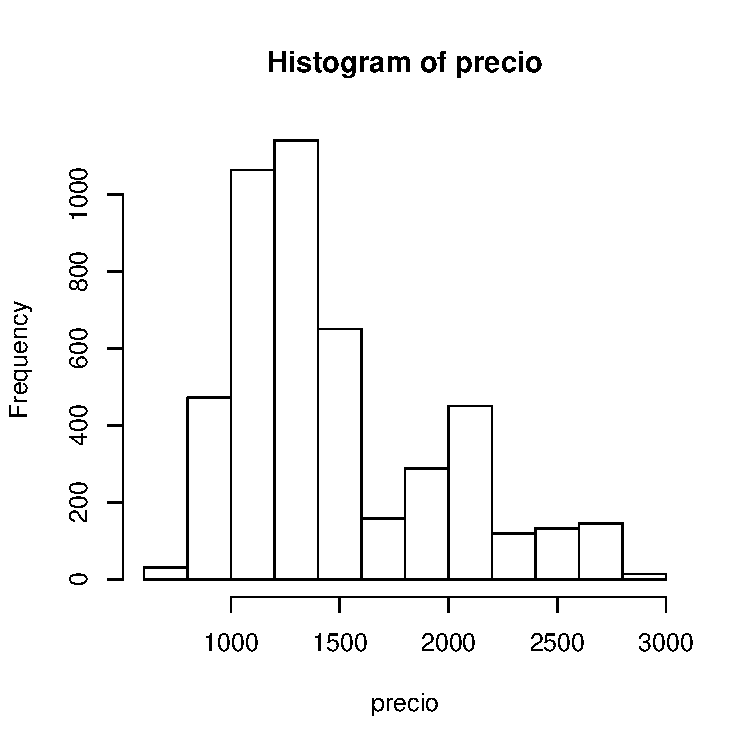
\includegraphics[width=\linewidth]{hist_precio_sp.pdf}}
	\caption{Histograma de los precios de la Bolsa de NY}\label{figura3}
\end{figure}
%\end{frame}

%---------------------------------------------------------
%---------------------Slide 14 --------------------------
%\begin{frame}
%\frametitle{Ejemplo 2: Series temporales financieras}
\pagebreak
Los retornos de los precios si parecen normales~\ref{figura4}, lo cual constituye una propiedad deseable para el an\'alisis estad\'\i{}stico.\\
\begin{figure}[H]
	\centering
	\textbf{Ejemplo 2: Histograma de los Precios}\par\medskip
	\fcolorbox{green}{blue}{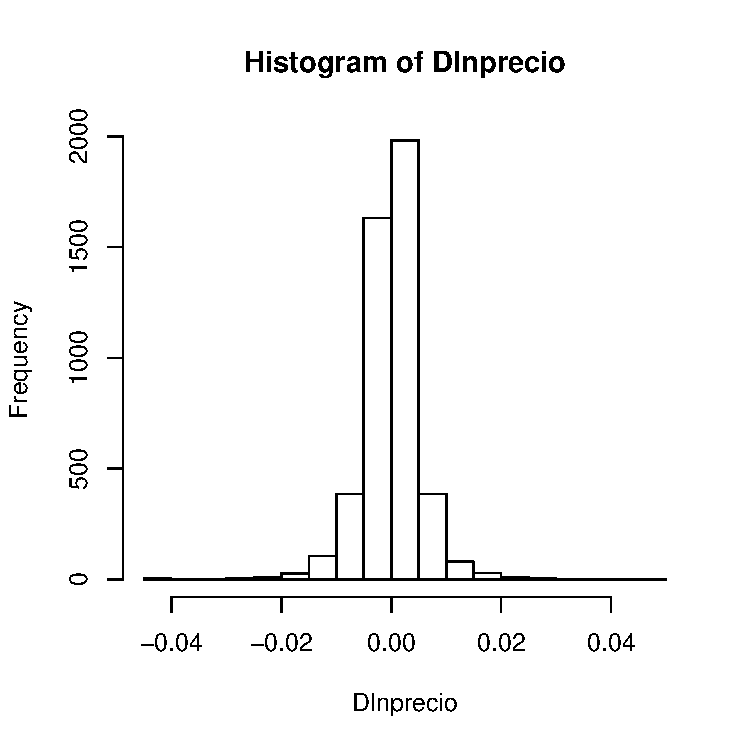
\includegraphics[width=\linewidth]{hist_dlnprecio_sp.pdf}}
	\caption{Histograma de los retornos de la Bolsa de NY}\label{figura4}
\end{figure}
%\end{frame}

%\end{section}
%---------------------------------------------------------
%---------------------Slide 15 --------------------------
%\begin{frame}
%\frametitle{Ejemplo 2: Series temporales financieras}
\begin{figure}[H]
	\centering
	\textbf{Ejemplo 2: Histograma de los Precios}\par\medskip
	\fcolorbox{green}{blue}{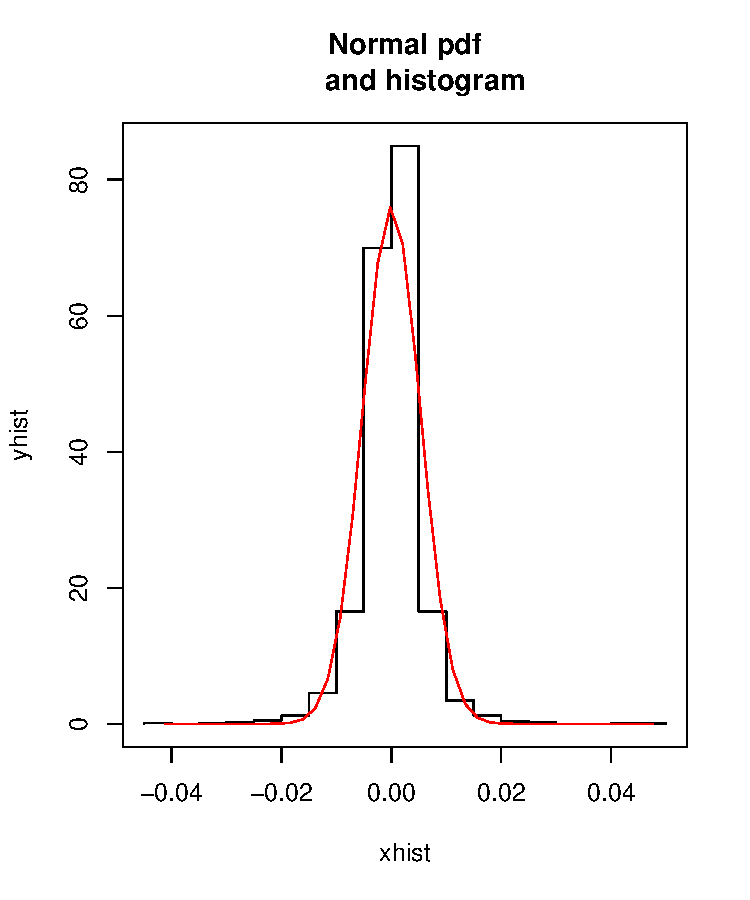
\includegraphics[width=\linewidth]{normal_hist_Dlnprice_sp.pdf}}
	\caption{Linea negra:Histograma de las diferencias de los log-precios de la Bolsa de NY. Linea roja: ajuste de la distribución normal segúun media y desviación estandar de la muestra. Shapiro-Wilk normality test / data:  Dlnprecio / W = 0.90927, p-value $<$ 2.2e-16.}\label{figura5}
\end{figure}
%Shapiro-Wilk normality test
%data:  Dlnprecio
%W = 0.90927, p-value $<$ 2.2e-16.
%\end{frame}

%---------------------------------------------------------
%---------------------Slide 16 --------------------------
%\begin{frame}
%\frametitle{Ejemplo 2: Series temporales financieras}
%
%\only<1|handout:1>{
	%\begin{exampleblock}{C\'odigo en R}
%		h $<-$ hist(Dlnprecio,breaks=15)\\
%		xhist $<-$ c(min(h\$breaks),h\$breaks)\\
%		yhist $<-$ c(0,h\$density,0)\\
%		xfit $<-$ seq(min(Dlnprecio),max(Dlnprecio),length=40)\\
%		yfit $<-$ dnorm(xfit,mean=mean(Dlnprecio),sd=sd(Dlnprecio))\\
%		plot(xhist,yhist,type="s",ylim=c(0,max(yhist,yfit)), main=``Normal pdf and histogram")\\
%		lines(xfit,yfit, col=``red")\\
%		shapiro.test(Dlnprecio)
	%\end{exampleblock}
%}
%\end{frame}
\pagebreak
\lstset{caption = Código R de histograma y ajuste de curva normal,framexleftmargin=5mm, frame=shadowbox, rulesepcolor=\color{green}}
\begin{lstlisting}[title={‘Código R de histograma y ajuste de curva normal’},basicstyle=\ttfamily]{}
h <- hist(Dlnprecio,breaks=15)
xhist <- c(min(h$breaks),h$breaks)
yhist <- c(0,h$density,0)
xfit <- seq(min(Dlnprecio),max(Dlnprecio),length=40)
yfit <- dnorm(xfit,mean=mean(Dlnprecio),sd=sd(Dlnprecio))
plot(xhist,yhist,type="s",ylim=c(0,max(yhist,yfit)), 
	main="Normal pdf and histogram")
lines(xfit,yfit, col="red")
shapiro.test(Dlnprecio)
\end{lstlisting}

%---------------------------------------------------------
%---------------------Slide 17 --------------------------
%\begin{section}{Modelamiento estad\'istico de las series de tiempo}
\section{Modelamiento estad\'istico de las series de tiempo}
%	\begin{frame}
%	\frametitle{Modelos estad\'isticos de series de tiempo}
	Para poder modelar los datos, que aparentemente fluct\'uan de forma aleatoria a lo largo del tiempo, suponemos que una serie temporal se define como una colecci\'on de variables aleatorias. 
	\\
	Por ejemplo, podemos modelar  una serie temporal como una secuencia de variables aleatorias, $x_1, x_2, x_3,...$, donde la variable aleatoria $x_1$ denota el valor tomado por la serie en el primer punto de tiempo, la variable $x_2$  denota el valor para el segundo per\'\i{}odo de tiempo, y as\'\i{} sucesivamente. 
	\\
	En general, una colecci\'on de variables aleatorias,  $\{x_t\}$, indexada por t se conoce como proceso estoc\'astico. En este texto, $t$ ser\'a t\'\i{}picamente discreto y variar\'a sobre los enteros $t = 0, \pm1, \pm2,,.... $, o alg\'un subconjunto de los enteros. Los valores observados en un proceso estoc\'astico se conocen como la realizaci\'on del proceso estoc\'astico.	
%\end{frame}
%---------------------------------------------------------
%---------------------Slide 18 --------------------------
%\begin{frame}
%\frametitle{Ruido blanco - White Noise}
\subsection{Ruido blanco - White Noise}
Una serie de tiempo muy utilizada es aquella representada por una colecci\'on de variables aleatorias no correlacionadas, $\epsilon_t$, con media $0$ y varianza finita $\sigma^2_\epsilon$. Las series temporales generadas a partir de variables no correlacionadas se utilizan por ejemplo para modelar el ruido en aplicaciones de ingenier\'\i{}a, donde se denomina ruido blanco. A veces denotaremos este proceso como $\epsilon_t$$\sim$$\epsilon_n (0, \sigma^2_\epsilon)$. La designaci\'on de "blanco" se origina de la analog\'\i{}a con la luz blanca e indica que todas las posibles oscilaciones peri\'odicas est\'an presentes con la misma fuerza.

%\end{frame}
%---------------------------------------------------------
%---------------------Slide 19 --------------------------
%\begin{frame}
%\frametitle{Ruido blanco - White Noise}

\begin{itemize}
	\item En ocasiones, tambi\'en requeriremos que el ruido sea independiente y tenga una distribuci\'on id\'entica (iid) de variables aleatorias con media 0 y varianza $\sigma^2_\epsilon$. Distinguiremos este caso diciendo ruido blanco independiente, o escribiendo $\epsilon_t$ $\sim$ $iid (0, \sigma^2_\epsilon)$. 
	\item Otra serie de ruido blanco particularmente \'util es el ruido blanco gaussiano, en el que las $w_t$ son variables aleatorias normales independientes, con media $0$ y varianza $\sigma^2_\epsilon$; o m\'as sucintamente, $\epsilon_t \sim iid \hspace{0.1cm}N(0, \sigma^2_\epsilon)$. 
	\item La figura siguiente muestra una colecci\'on de 500 de estas variables aleatorias, con $\sigma^2_\epsilon=1$, trazadas en el orden en que se dibujaron.
\end{itemize}

%\end{frame}
%---------------------------------------------------------
%---------------------Slide 20 --------------------------
%\begin{frame}
%\frametitle{Ruido blanco - White Noise}
%
%\only<1|handout:1>{
%	\begin{exampleblock}{C\'odigo en R}
%		set.seed(154) \\
%		w = rnorm(200,0,1) \\
%		plot.ts(w, ylim=c(-3,3), main="White Noise") \\
%	\end{exampleblock}
%}
%\begin{figure}[t!]
%	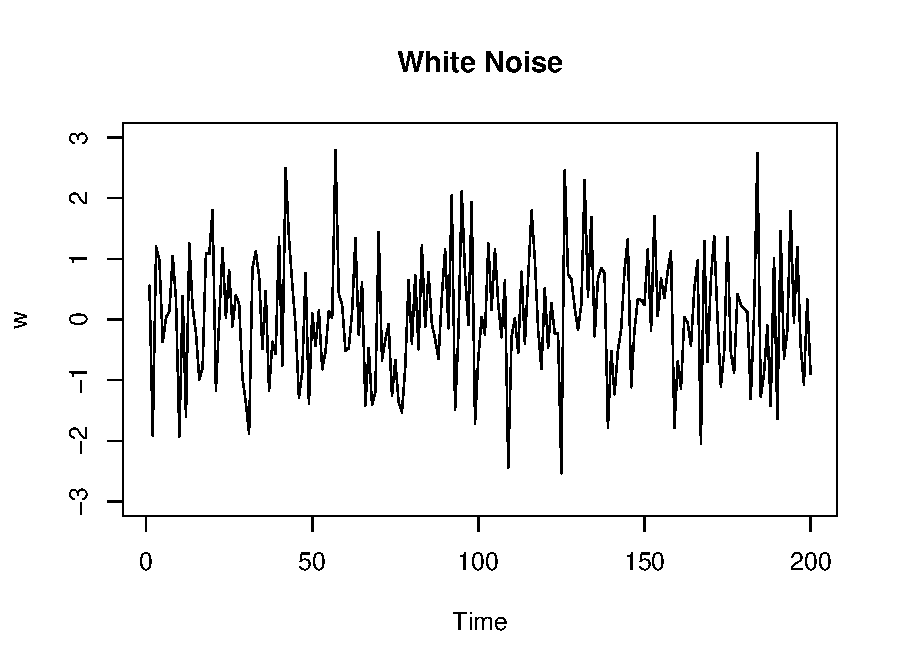
\includegraphics[scale=0.3]{white_noise.pdf}
%\end{figure}
%
%\end{frame}
\lstset{caption = Código R para generar Ruido blanco,framexleftmargin=5mm, frame=shadowbox, rulesepcolor=\color{green}}
\begin{lstlisting}[title={‘Código R para generar Ruido blanco’},basicstyle=\ttfamily]{}
set.seed(154)
w = rnorm(200,0,1)
plot.ts(w, ylim=c(-3,3), main="White Noise")
\end{lstlisting}\label{codigoRuidoBlanco}

\begin{figure}[H]
	\centering
	\textbf{Ruido blanco - White Noise}\par\medskip
	\fcolorbox{green}{blue}{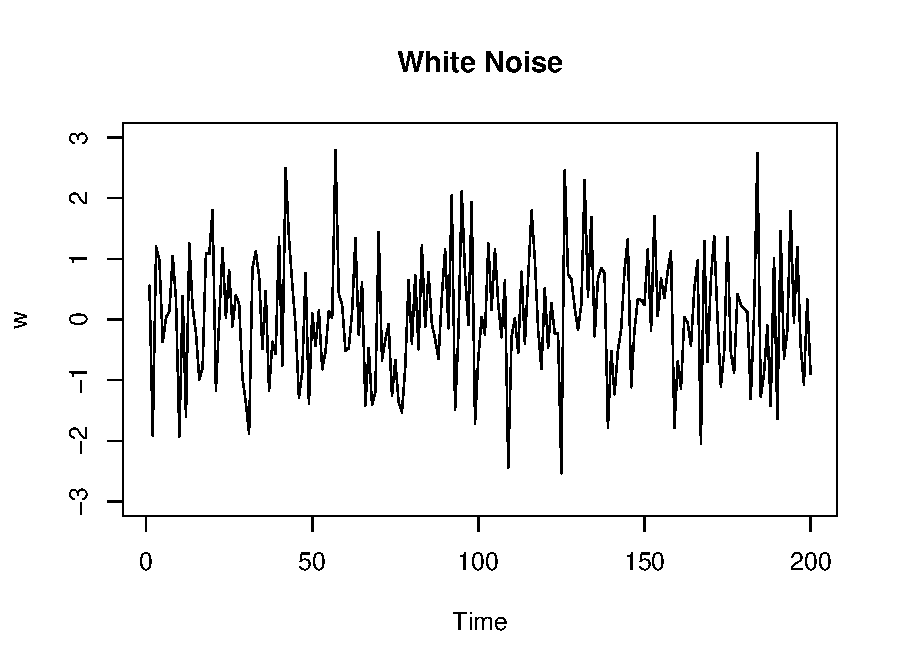
\includegraphics[width=\linewidth]{white_noise.pdf}}
	\caption{Ruido blanco - White Noise}\label{figura6}
\end{figure}

%---------------------------------------------------------
%---------------------Slide 21 --------------------------
%\begin{frame}
%\frametitle{Caminata Aleatoria - Random Walk}
\subsection{Caminata Aleatoria - Random Walk}

Un ejemplo simple para modelar una serie temporal estoc\'astica con tendencia (no estacionaria) es una caminata aleatoria con deriva (Random Walk with drift):

\begin{equation*}
x_t = \delta + x_{t-1} + \epsilon_t 
\end{equation*}

para $t = 1, 2,. . .$, con una condici\'on inicial $x_0 = 0$, y donde $\epsilon_t$ es ruido blanco. La constante $\delta$ se denomina deriva (drift), y cuando $\delta=0$, se llama simplemente una caminata aleatoria. El t\'ermino caminata aleatoria proviene del hecho de que, cuando $\delta=0$, el valor de la serie de tiempo en el tiempo $t$, es el valor de la serie en el tiempo $t - 1$ m\'as un movimiento completamente aleatorio determinado por $\epsilon_t$. 
%\end{frame}

%---------------------------------------------------------
%---------------------Slide 22 --------------------------
%\begin{frame}
%\frametitle{Caminata Aleatoria - Random Walk}

Tenga en cuenta que podemos reescribir la ecuaci\'on anterior como una suma acumulativa de las variables de ruido blanco. Es decir,

\begin{equation*}
x_t = \delta t + \sum_{j=1}^{t} \epsilon_t 
\end{equation*}

%\end{frame}
%---------------------------------------------------------
%---------------------Slide 23 --------------------------
%\begin{frame}
%\frametitle{Caminata Aleatoria - Random Walk}

%\only<1|handout:1>{
%	\begin{exampleblock}{C\'odigo en R}
%		set.seed(154) \\
%		w = rnorm(200,0,1) \\
%		x = cumsum(w) \\
%		wd = w + 0.2 \\
%		xd = cumsum(wd) \\
%		plot.ts(xd, ylim=c(-5,55), main=``random walk") \\
%		lines(x) \\
%		lines(0.2*(1:200), lty=``dashed") \\
%	\end{exampleblock}
%}
%\end{frame}
\lstset{caption = Código R para generar Caminata Aleatoria,framexleftmargin=5mm, frame=shadowbox, rulesepcolor=\color{green}}
\begin{lstlisting}[title={‘Código R para generar Caminata Aleatoria’},basicstyle=\ttfamily]{}
set.seed(154)
w = rnorm(200,0,1)
x = cumsum(w)
wd = w + 0.2
xd = cumsum(wd)
plot.ts(xd, ylim=c(-5,55), main="random walk")
lines(x)
lines(0.2*(1:200), lty="dashed")
\end{lstlisting}\label{codigoCaminataAleatoria}

%---------------------------------------------------------
%---------------------Slide 24 --------------------------
%\begin{frame}
%\frametitle{Caminata Aleatoria - Random Walk}

\begin{figure}[H]
	\centering
	\textbf{Caminata aleatoria}\par\medskip
	\fcolorbox{green}{blue}{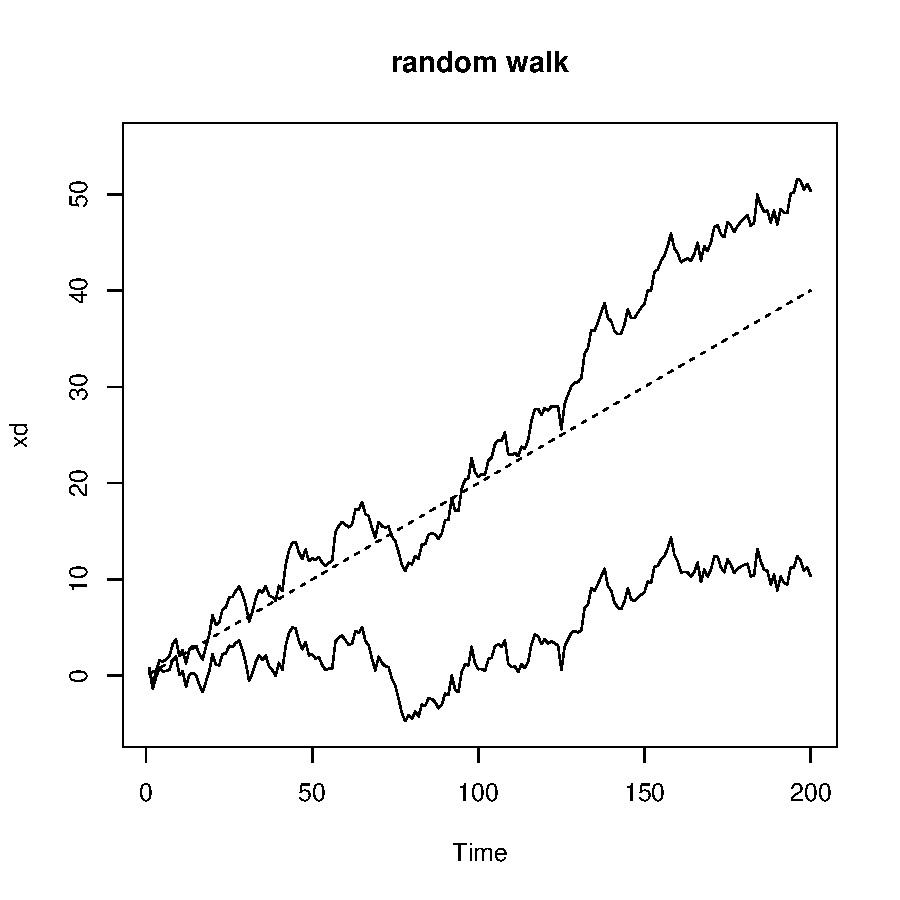
\includegraphics[width=\linewidth]{random_walk.pdf}}
%	\textbf{Random Walk}\par\medskip
%	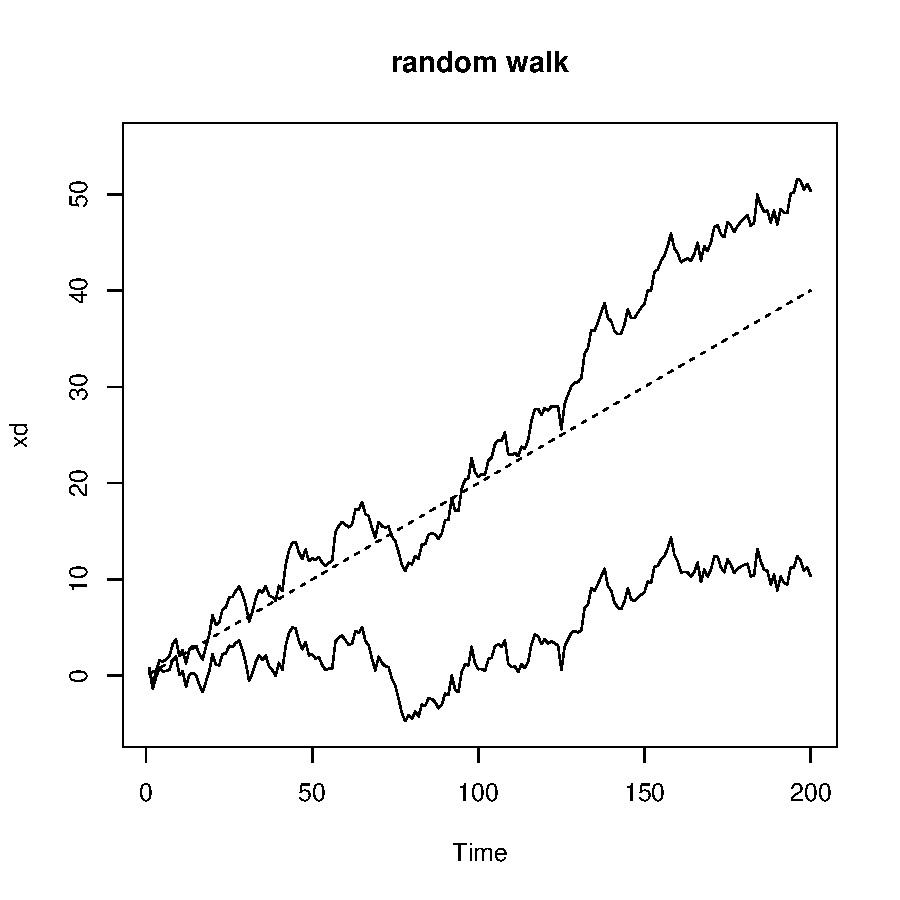
\includegraphics[scale=0.6]{random_walk.pdf}
	\caption{Caminata Aleatoria - Random walk, $\sigma_\epsilon$ = 1, with drift $\delta =0 .2$ (upper jagged line), without drift, $\delta = 0$ (lower jagged line), and a straight line with slope 0.2 (dashed line).}\label{figura7}
\end{figure}

%---------------------------------------------------------
%---------------------Slide 25 --------------------------
%\begin{frame}
%\frametitle{Promedios m\'oviles - Moving Averages}
\pagebreak\subsection{Promedios m\'oviles - Moving Averages}
Podr\'\i{}amos reemplazar la serie de ruido blanco $\epsilon_t$ por un promedio m\'ovil que suavice la serie. Por ejemplo, considere reemplazar $\epsilon_t$ por un promedio de su valor actual y sus vecinos inmediatos en el pasado y futuro. Es decir:

\begin{equation*}
v_t = 1/3 (\epsilon_{t-1} + \epsilon_t + \epsilon_{t+1})
\end{equation*}

Como veremos en el siguiente ejemplo, los promedios m\'oviles producen una versi\'on m\'as suave que la serie original, lo que refleja el hecho de que las oscilaciones m\'as lentas llegan a ser m\'as evidentes, y se eliminan algunas de las oscilaciones m\'as r\'apidas. 

%\end{frame}
%---------------------------------------------------------
%---------------------Slide 26 --------------------------
%\begin{frame}
%\frametitle{Promedios m\'oviles - Moving Averages}

%\only<1|handout:1>{
%	\begin{exampleblock}{C\'odigo en R}
%		w = rnorm(500,0,1) ; v = filter(w, sides=2, rep(1/3,3)) 
%		par(mfrow=c(2,1))\\
%		plot.ts(w, main=``white noise"); plot.ts(v, main=``moving average")\\
%	\end{exampleblock}
%}
\lstset{caption = Código R para generar Promedios móviles,framexleftmargin=5mm, frame=shadowbox, rulesepcolor=\color{green}}
\begin{lstlisting}[title={‘Código R para generar Moving Averages’},basicstyle=\ttfamily]{}
w = rnorm(500,0,1) ; v = filter(w, sides=2, rep(1/3,3))
par(mfrow=c(2,1))
plot.ts(w, main="white noise")
plot.ts(v, main="moving average")
\end{lstlisting}\label{movingAverage}
\begin{figure}[H]
	\centering
	\textbf{Medias móviles}\par\medskip
	\fcolorbox{green}{blue}{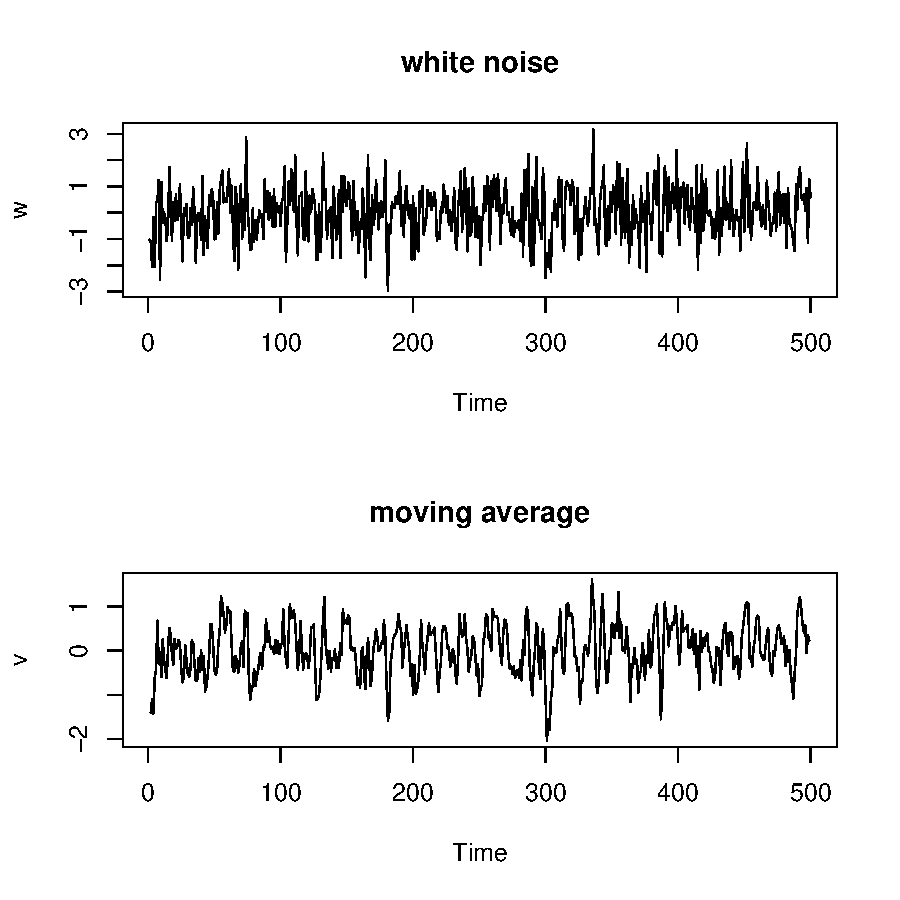
\includegraphics[width=\linewidth]{moving_average.pdf}}
%	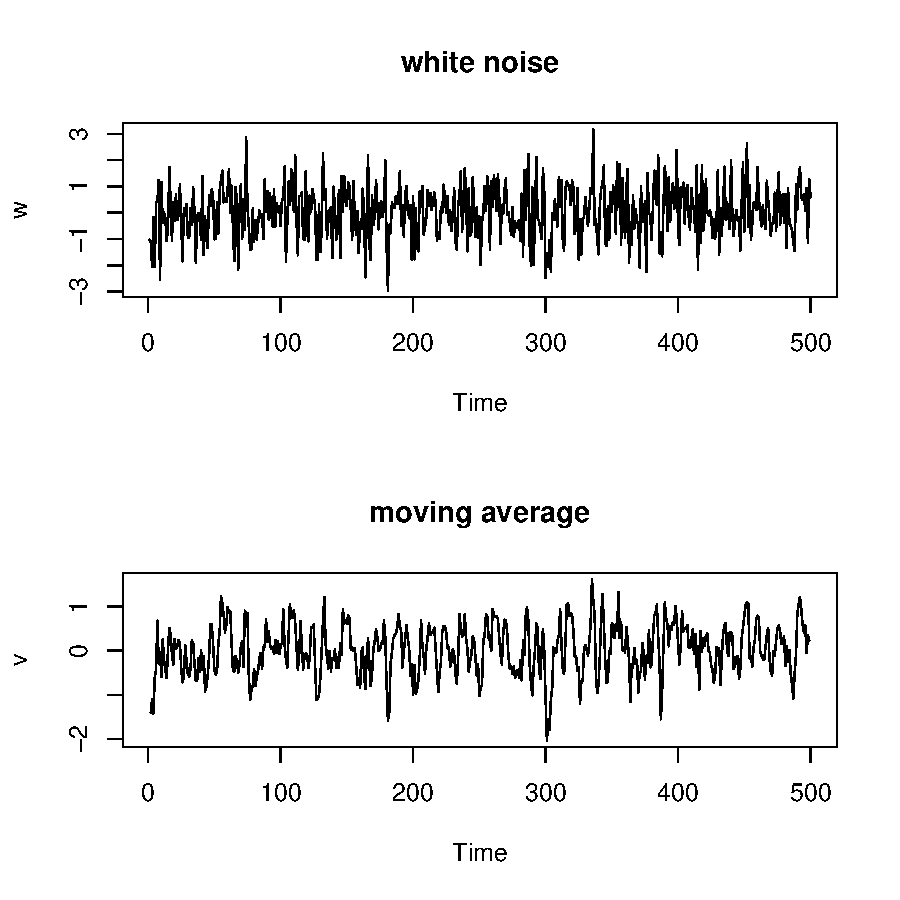
\includegraphics[scale=0.7]{moving_average.pdf}
	\caption{Promedios Móviles - Moving Averages}\label{figura8}
\end{figure}

%\end{frame}



%\end{frame}
%---------------------------------------------------------
%---------------------Slide 27 --------------------------
%\begin{frame}
%\frametitle{Autorregresiones - Autoregressions}
\subsection{Autorregresiones - Autoregressions}
Supongamos nuevamente que consideramos la serie de ruido blanco $w_t$ como entrada, y calculamos la salida usando una ecuaci\'on de segundo orden, es decir:

\begin{equation*}
x_t = x_{t-1} - 0.9 x_{t-2} + \epsilon_t
\end{equation*}

Esta ecuaci\'on representa una regresi\'on o predicci\'on del valor actual $x_t$ de una serie temporal en funci\'on de los dos valores anteriores de la serie, es por esto que utilizamos el nombre de autoregresi\'on.

%\end{frame}

%---------------------------------------------------------
%---------------------Slide 28 --------------------------
%\begin{frame}
%\frametitle{Autorregresiones - Autoregressions}

%\only<1|handout:1>{
%\begin{exampleblock}{C\'odigo en R}
%	w = rnorm(550,0,1) ; x = filter(w, filter=c(1,-.9), method= ``recursive")[-(1:50)]\\
%	plot.ts(x, main= ``autoregression")
%\end{exampleblock}
%}
\lstset{caption = Código R para generar Auto regresiones,framexleftmargin=5mm, frame=shadowbox, rulesepcolor=\color{green}}
\begin{lstlisting}[title={‘Código R para generar Autoregresions’},basicstyle=\ttfamily]{}
w = rnorm(550,0,1) ; 
x = filter(w, filter=c(1,-.9), method="recursive")[-(1:50)]
plot.ts(x, main= "autoregression")
\end{lstlisting}\label{autoregression}
\begin{figure}[H]
	\centering
	\textbf{Autorregresiones}\par\medskip
	\fcolorbox{green}{blue}{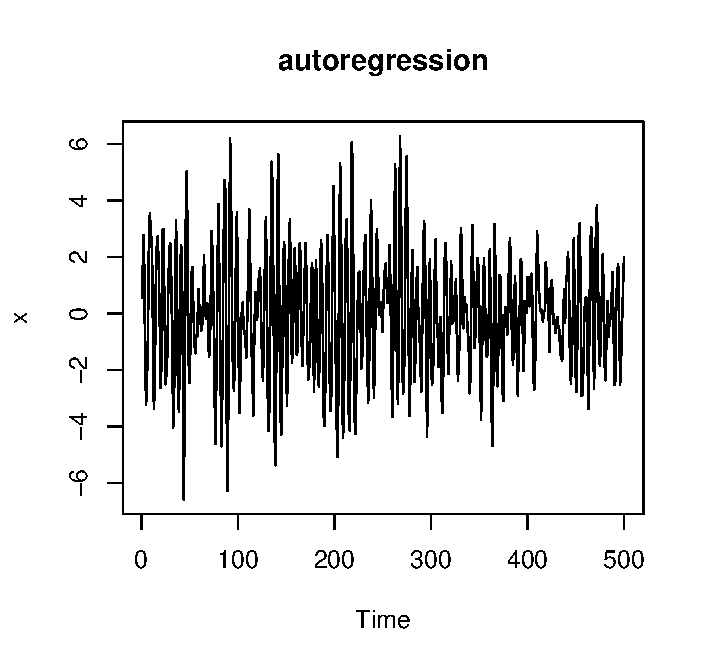
\includegraphics[width=\linewidth]{autoregression.pdf}}
%	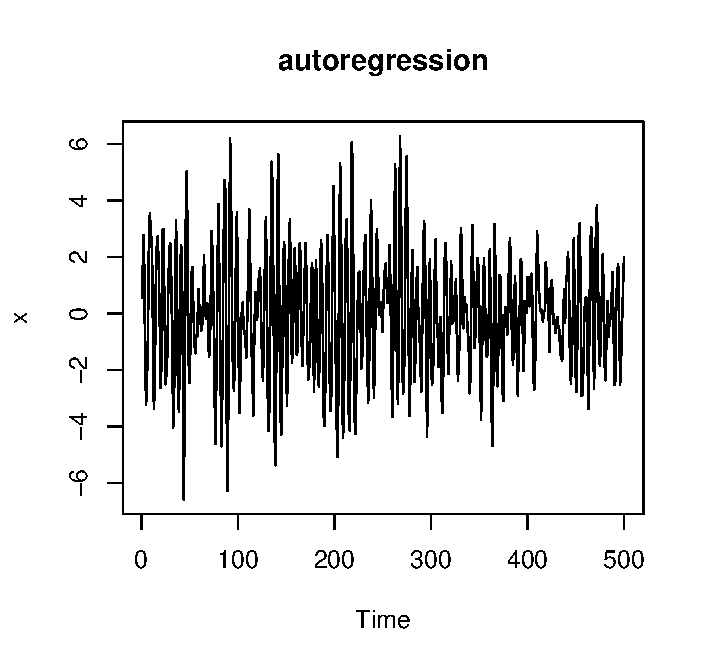
\includegraphics[scale=0.7]{autoregression.pdf}
	\caption{Autorregresiones - Autoregressions}\label{figura9}
\end{figure}

%---------------------------------------------------------
%---------------------Slide 29 --------------------------
\pagebreak\section{Descomposici\'on de las series de tiempo}
%	\begin{frame}
%	\frametitle{Descomposici\'on de las series de tiempo}	
Las series de tiempo usualmente se descomponen en:
	\begin{itemize}
		\item Una tendencia (trend) $T_t$. 
		\item Un componente estacional (seasonal) $S_t $.
		\item Un elemento irregular (irregular) $I_t$.
	\end{itemize}
	\vspace{5mm}
Por ejemplo:
	\begin{center}
		\vspace{3mm}
		$T_t=2+0.1 t$; \\
		\vspace{3mm}
		$S_t = 6.5 cos (\pi/60)$; \\
		\vspace{3mm}
		y $I_t\sim$ $N(\mu=0, \sigma^2=0.5)$. 
	\end{center}
%---------------------------------------------------------
%---------------------Slide 30 --------------------------
%\begin{frame}
%\frametitle{Descomposici\'on de las series de tiempo}
%
%\only<1|handout:1>{
%	\begin{exampleblock}{C\'odigo en R}
%		rm(list=ls())\\
%		$t = 2 + 0.1*1:500$\\
%		$s = 6.5*cos(pi*1:500/90)$\\
%		set.seed(154) \\
%		$i = rnorm(500,0,5)$\\
%		$plot.ts(s+t+i)$\\
%	\end{exampleblock}
%}
%\end{frame}
\lstset{caption = Código R para descomponer serie de tiempo,framexleftmargin=5mm, frame=shadowbox, rulesepcolor=\color{green}}
\begin{lstlisting}[title={‘Código R para descomponer serie de tiempo’},basicstyle=\ttfamily]{}
t = 2 + 0.1 * 1:500
s = 6.5 * cos(pi * 1:500/90)
set.seed(154)
i = rnorm(500, 0, 5)
plot.ts(s + t + i)
\end{lstlisting}\label{descomposicionTS}

%---------------------------------------------------------
%---------------------Slide 31 --------------------------
%\begin{frame}
%\frametitle{Descomposici\'on de las series de tiempo}
\begin{figure}[H]
	\centering
	\textbf{Componentes de uuna Serie de Tiempo}\par\medskip
	\fcolorbox{green}{blue}{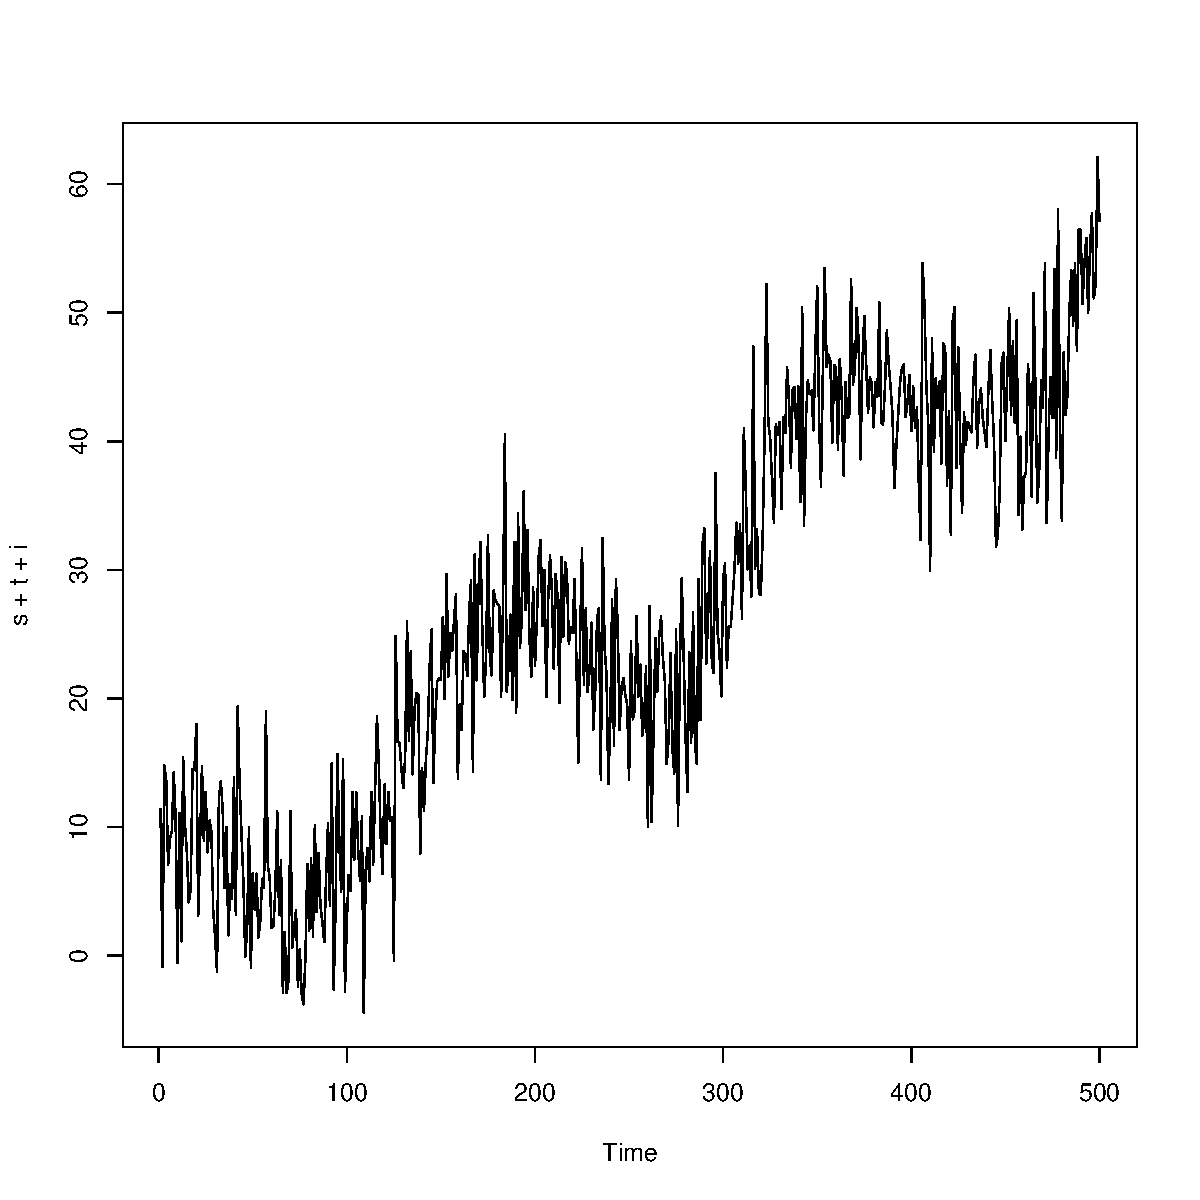
\includegraphics[width=\linewidth]{time_series.pdf}}
%	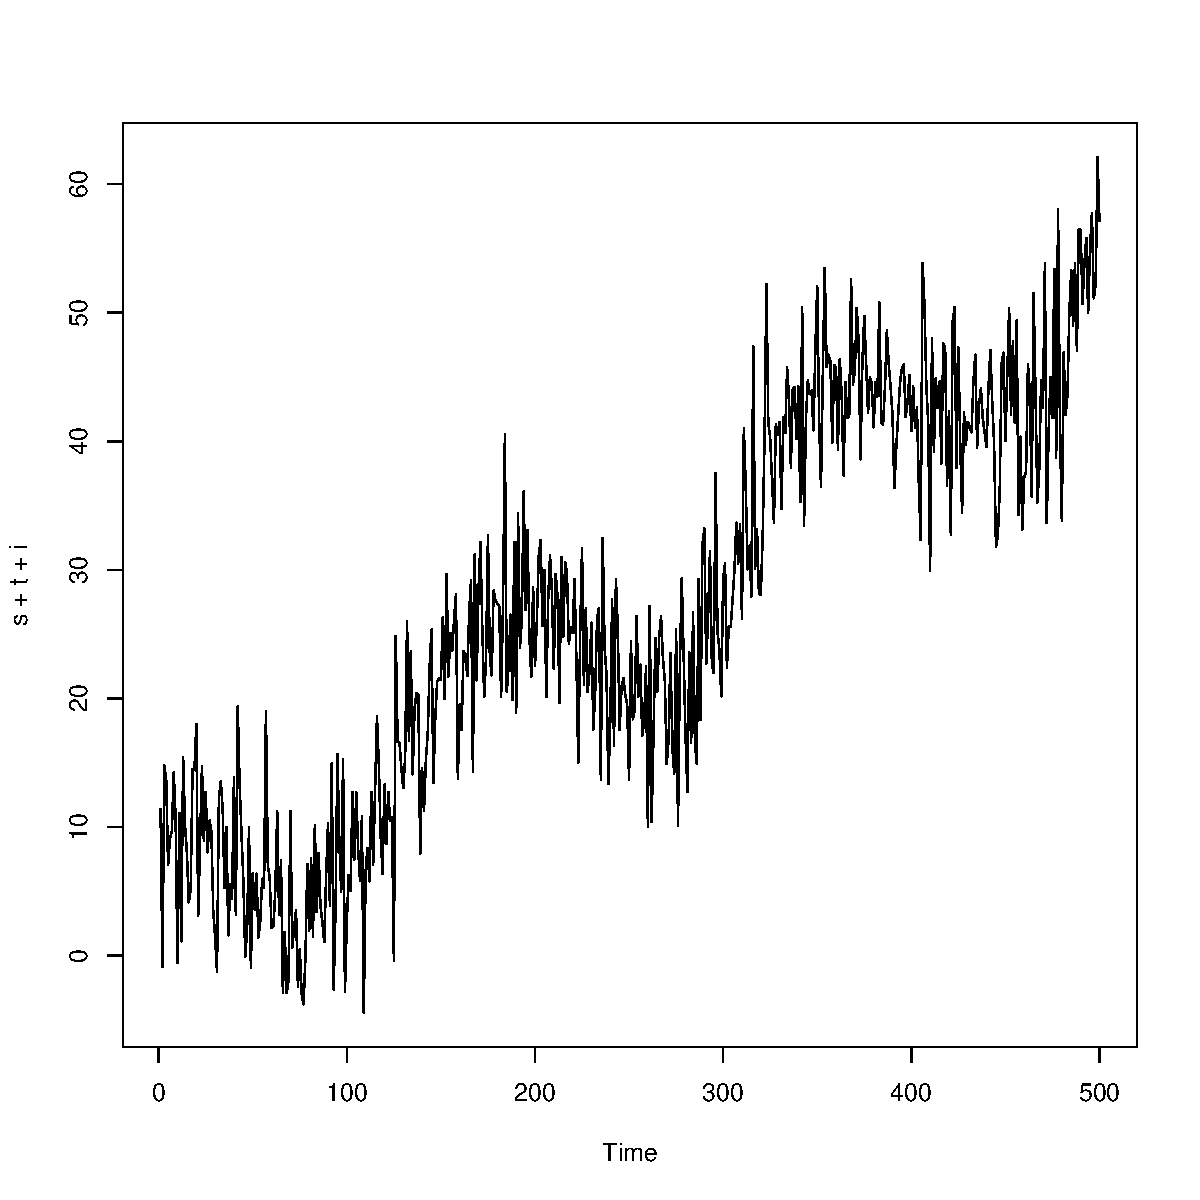
\includegraphics[scale=0.5]{time_series.pdf}
	\caption{Serie de tiempo con sus componentes T, S e I.}\label{figura10}
\end{figure}
%\end{frame}
%---------------------------------------------------------
%---------------------Slide 32 --------------------------
%\begin{frame}
%\frametitle{Descomposici\'on de las series de tiempo}

En general, las series de tiempo pueden contener uno o combinaci\'on de todos los elementos antes se\~nalados, ya sea de manera aditiva o multiplicativa:

\begin{equation*}
x_t = T_t + S_t + I_t
\end{equation*}

\begin{equation*}
x_t = T_t * S_t * I_t
\end{equation*}

\begin{itemize}
\item La primera especificaci\'on se caracteriza por tener cada componente de forma independiente, lo que posibilita descomponer la serie en una suma de los tres factores.
\item  La segunda, por otra parte, surge cuando la tendencia $(T_t)$, estacionalidad $(S_t)$, y irregularidad $(I_t)$ son dependientes entre si.
\end{itemize}

%\end{frame}

%---------------------------------------------------------
%---------------------Slide 33 --------------------------
%\begin{frame}
%\frametitle{Descomposici\'on de las series de tiempo}

En general, la tendencia cambia la media de la serie, mientras que el componente estacional posee un patr\'on que se repite, por ejemplo de manera mensual o trimestral. El componente irregular a pesar de no tener un patr\'on bien definido, puede ser pronosticada, de hecho, los pron\'osticos usan correlaciones con el componente irregular para realizar sus pron\'osticos. En per\'\i{}odos m\'as largos sin embargo, el componente irregular exhibe una tendencia de reversi\'on a cero.\\
El pron\'ostico de series de tiempo pretende entonces predecir cada uno de \'estos componentes de manera individual. Como vimos, el pron\'ostico global de la series de tiempo agrupa de forma aditiva o multiplicativa cada uno de dichos componentes.

%---------------------------------------------------------
%---------------------Slide 34 --------------------------
%\begin{frame}
%\frametitle{Descomposici\'on Tendencia\\
\subsection{Descomposici\'on Tendencia - Filtro Hodrick -Prescott}

\begin{itemize}
	\item En econom\'\i{}a, el filtro Hodrick-Prescott (HP) permite separar para $x_t$  los componentes tendencial y c\'\i{}clico.
	\item Este m\'etodo consiste en obtener una serie suavizada $S_t$ a partir de la original $x_t$, mediante una soluci\'on al problema de optimizaci\'on sugerido en la siguiente ecuaci\'on. Una vez resuelto, permite estimar tanto el ciclo como la tendencia de la serie.
\end{itemize}

\begin{equation*}
min \sum_{t=1}^{n} \left(x_t -S_t\right)^2 + \lambda \sum_{t=2}^{n-1} \left[ \left(S_{t+1}-S_t\right)-\left(S_t-S_{t-1}\right)\right]^2
\end{equation*}

\begin{itemize}
	\item Los valores sugeridos para $\lambda$ dependen de la periodicidad de $x_t$, y son: 14400 (mensual), 1600 (trimestral) y 100 (anual). Por otra parte, una vez obtenido el componente c\'\i{}clico $ \left(x_t -S_t\right)$, a partir del filtro HP, puede ser interpretada como la brecha existente entre su valor real $x_t$ y potencial $S_t$.
\end{itemize}

%---------------------------------------------------------
%---------------------Slide 35 --------------------------
%\begin{frame}
%\frametitle{Descomposici\'on componente estacional\\ 	Transformaciones de Diferencias}
\subsection{Descomposici\'on componente estacional - Transformaciones de Diferencias}

La transformaciones de diferencias se usan para capturar el componente estacional de la serie:

Una primera diferencia es definida como:

\begin{equation*}
\triangle x_t = (x_t - x_{t-1})
\end{equation*}

An\'alogamente, la segunda diferencia es definida como:

\begin{equation*}
\triangle^2x_t = (x_t - x_{t-1})-(x_{t-1} - x_{t-2})
\end{equation*}
Anteriormente vimos que la primera diferencia del logaritmo, se pod\'\i{}a interpretar como el cambio porcentual de la variable, logrando la simetr\'\i{}a del precio de las acciones.

%---------------------------------------------------------

%---------------------Slide 36 --------------------------
%\begin{frame}
%\frametitle{Descomposici\'on componente estacional\\
%	Variables Dummy}
\subsection{Descomposici\'on componente estacional - Variables Dummy}
Una variable dummy, D, es una variable binaria que toma la siguiente forma:

\begin{itemize}
	\item D=1  si la observaci\'on tiene caracter\'\i{}sticas espec\'\i{}ficas.
	\item D=0 si no las tiene.
\end{itemize}

Por ejemplo:

\begin{equation*}
x_t  = \beta_0 + \beta_1 z_t + \beta_2 D + \beta_3 D z_t
\end{equation*}

\begin{equation*}
D=1 => x_t  = (\beta_0 + \beta_2) + (\beta_1 + \beta_3) z_t
\end{equation*}

\begin{equation*}
D=0 => x_t  = \beta_0 + \beta_1 z_t
\end{equation*}

Las variables dummy pueden ser usadas para cambiar la pendiente y/o intercepto en un modelo lineal, lo cual permite capturar la estacionalidad en la serie, por ejemplo con variables dummys por trimestre o temporada.
%---------------------------------------------------------
%---------------------Slide 37 --------------------------
%\begin{section}{Medidas de dependencia}
%	\begin{frame}
%	\frametitle{Medidas de dependencia}
\pagebreak\section{Medidas de dependencia}
	Como vimos anteriormente, una serie de tiempo puede ser vista como una colecci\'on de n variables aleatorias en puntos de tiempo enteros arbitrarios $t_1, t_2,\cdots, t_n$, para cualquier entero positivo se cuenta con una funci\'on de distribuci\'on conjunta, evaluada como la probabilidad que los valores de las series sean conjuntamente menores que n constantes, $c_1, c_2,\cdots, c_n$, i.e.:
	\begin{equation*}
	F(c_1, c_2,\cdots, c_n) =  P(x_{t_1},\le c_1, x_{t_2} 	\le c_2,\cdots x_{t_n} \le c_n)
	\end{equation*}

%\end{frame}
%---------------------------------------------------------
%---------------------Slide 38 --------------------------
%\begin{frame}
%\frametitle{Medidas de dependencia}

Desafortunadamente, la funci\'on de distribuci\'on multinomial no puede usualmente ser escrita f\'acilmente a menos que las variables sean conjuntamente normales, en cual caso la densidad conjunta presenta la forma:
\begin{equation*}
f(\textbf{x}) = (2\pi)^{-2/n}\mid\Gamma\mid^{-1/2} exp \{ -1/2  (\textbf{x} - \mu)' \Gamma^{-1}\ (\textbf{x} - \mu)\}
\end{equation*}

donde $\mid\cdot\mid$ indica determinante y $\Gamma$ la matriz de covarianza.\\
Aunque la funci\'on de distribuci\'on conjunta permite describir la data completamente, su manipulaci\'on es muy compleja, y su despliegue gr\'afico imposible.
%\end{frame}
%---------------------------------------------------------
%---------------------Slide 39 --------------------------
%\begin{frame}
%\frametitle{Medidas de dependencia}

Las funciones de distribuci\'on marginales:
\begin{equation*}
F_t(x) = P\{x_t \le x\}
\end{equation*}

o la correspondiente funci\'on de densidad marginal:\\
\begin{equation*}
f_t(x) = \frac{\partial F_t(x)}{\partial x} 
\end{equation*}
\\
Cuando \'estas existen, proveen informaci\'on valiosa para examinar el comportamiento marginal de la serie.
\\
Si $x_t$ es Gausiana con media $\mu_t$ y varianza $\sigma_t^2$, $x_t$ $\sim$ $N(\mu_t,\sigma_t^2)$, la densidad marginal esta dada por:

\begin{equation*}
f_t(x) = \frac{1}{\sigma_t \sqrt{2 \pi}} exp  ( -  \frac{1}{2 \sigma_t^2}  (\textbf{x} - \mu_t)^2 )
\end{equation*}
%\end{frame}

%---------------------------------------------------------
%---------------------Slide 40 --------------------------
%\begin{frame}
%\frametitle{Medidas de dependencia}

La funci\'on de media, conocida en estad\'\i{}stica como el primer momento central, est\'a definida como:
\vspace{5mm}

%\only<1|handout:1>{
%\begin{block}{Definici\'on: Funci\'on de Media}
%	\begin{equation*}
%	\mu_{xt} = E(x_t)= \int^{+\infty}_{-\infty} x f_t(x)dx
%	\end{equation*}
%\end{block}
%}
%\section{Definition}
\begin{definition}\label{def:def1}
	\textbf{Definici\'on: Funci\'on de Media:}
	\begin{equation*}
	\mu_{xt} = E(x_t)= \int^{+\infty}_{-\infty} x f_t(x)dx
	\end{equation*} 

\end{definition}

Si existe, E denota el operador de valor esperado.

%\end{frame}

%---------------------------------------------------------
%---------------------Slide 41 --------------------------
%\begin{frame}
%\frametitle{Medidas de dependencia}

La funci\'on de autocovarianza, conocida en estad\'\i{}stica como el segundo momento central, est\'a definida como:
\vspace{5mm}

%\only<1|handout:1>{
%\begin{block}{Definici\'on: Funci\'on de Autocovarianza}
%\begin{equation*}
%\gamma_{x}(s,t) = cov(x_s, x_t) = E[(x_s - \mu_s)(x_t - \mu_t)] 
%\end{equation*}
%\end{block}
%}
%\section{Definition}
\begin{definition}\label{def:def2}
	\textbf{Definici\'on: Funci\'on de Autocovarianza:} 
	\begin{equation*}
	\gamma_{x}(s,t) = cov(x_s, x_t) = E[(x_s - \mu_s)(x_t - \mu_t)] 
	\end{equation*}
\end{definition}

En este caso, $\gamma_{x}(s,t) = \gamma_{x}(t,s)$ para todos los puntos de $s$ y $t$. Si $\gamma(s,t)=0$ podemos asegurar que $x_s$ y $x_t$ no est\'an linealmente relacionadas. Por otro lado, si $x_s$ y $x_t$  son adem\'as normales bivariadas podemos asegurar que son independientes.
\\
Por \'ultimo, es claro que si $s = t$, la autocovarianza se reduce a la varianza
%\only<1|handout:1>{
%\begin{block}{Definici\'on: Funci\'on de Varianza}
%\begin{equation*}
%\gamma_{x}(t,t) = E[(x_t - \mu_t)^2] = var(x_t) 
%\end{equation*}
%\end{block}
%}
%\section{Definition}
\begin{definition}\label{def:def3}
	\textbf{Definici\'on: Funci\'on de Varianza:}
	\begin{equation*}
	\gamma_{x}(t,t) = E[(x_t - \mu_t)^2] = var(x_t) 
	\end{equation*} 
\end{definition} 



%\end{frame}

%---------------------------------------------------------
%---------------------Slide 42 --------------------------
%\begin{frame}
%\frametitle{Medidas de dependencia}

La Funci\'on de Autocorrelaci\'on, denotada por ACF (autocorrelation function),  mide la predictibilidad lineal de la serie en el tiempo t. Es decir, predecimos $x_t$, utilizando s\'olo el valor $x_s$. Suponiendo que ambas series tienen varianzas finitas, tenemos la siguiente definici\'on:

\vspace{5mm}

%\only<1|handout:1>{
%\begin{block}{Definici\'on: Funci\'on de Autocorrelaci\'on}
%\begin{equation*}
%\rho(s,t) = \frac{\gamma(s,t)}{ \sqrt{\gamma(s,s) \gamma(t,t)}}
%\end{equation*}
%\end{block}
%}
%\section{Definition}
\begin{definition}\label{def:def4}
	\textbf{Definici\'on: Funci\'on de Autocorrelaci\'on:} 
	\begin{equation*}
	\rho(s,t) = \frac{\gamma(s,t)}{ \sqrt{\gamma(s,s) \gamma(t,t)}}
	\end{equation*}
\end{definition} 

Se puede demostrar f\'acilmente que $-1 \le \rho(s,t) \le 1$. Si podemos predecir $x_t$ perfectamente a partir de $x_s$ a trav\'es de una relaci\'on lineal, $x_t = \beta_0 + \beta_1 x_s$, entonces la correlaci\'on ser\'a $+1$ cuando $\beta_1 > 0$, y $-1$ cuando $\beta_1 < 0$. \\
Por lo tanto, tenemos una medida aproximada de la capacidad de predecir la serie en el tiempo $t$ desde el valor en el tiempo $s$.

%\end{frame}

%---------------------------------------------------------
%---------------------Slide 43 --------------------------
%\begin{frame}
%\frametitle{Medidas de dependencia}

La funci\'on de covarianza cruzada entre dos series, $x_t$ e $y_t$, viene dada por:
\vspace{5mm}

%\only<1|handout:1>{
%\begin{block}{Definici\'on: Funci\'on de Covarianza Cruzada}
%\begin{equation*}
%\gamma_{xy} (s, t) = cov (x_s, y_t) = E [(x_s -\mu_{xs}) (y_t - \mu_{yt})].
%\end{equation*}
%\end{block}
%}
%\section{Definition}
\begin{definition}\label{def:def5}
	\textbf{Definici\'on: Funci\'on de Covarianza Cruzada:}
\begin{equation*}
\gamma_{xy} (s, t) = cov (x_s, y_t) = E [(x_s -\mu_{xs}) (y_t - \mu_{yt})].
\end{equation*}
\end{definition}
La funci\'on de correlaci\'on cruzada (CCF por su sigla en ingl\'es cross-correlation function) est\'a dada por:
\vspace{5mm}

%\only<1|handout:1>{
%\begin{block}{Definici\'on: Funci\'on de Correlaci\'on Cruzada}
%\begin{equation*}
%\rho_{xy} (s, t) = \frac{\gamma_{xy}(s,t)}{ \sqrt{\gamma_x(s,s) \gamma_y(t,t)}}
%\end{equation*}
%\end{block}
%}
%\section{Definition}
\begin{definition}\label{def:def6}
\textbf{Funci\'on de Correlaci\'on Cruzada:}
\begin{equation*}
\rho_{xy} (s, t) = \frac{\gamma_{xy}(s,t)}{ \sqrt{\gamma_x(s,s) \gamma_y(t,t)}}
\end{equation*}

\end{definition} 

%\end{frame}
%---------------------------------------------------------
%---------------------Slide 44 --------------------------
%\begin{frame}
%\frametitle{Medidas de dependencia}

Podemos extender f\'acilmente las formulaciones anteriores al caso de m\'as de dos series, por ejemplo, $x_{t1}, x_{t2},\cdots, x_{tr}$; es decir, series temporales multivariantes con $r$ componentes. Por ejemplo, la extensi\'on de (1.10) para el caso de covarianza cruzada ser\'\i{}a:

\begin{equation*}
\gamma_{xy} (j, k) = cov (x_{sj}, y_{sk}) = E [(x_s -\mu_{xs}) (y_{tj} - \mu_{y_{tk}})].
\end{equation*}

%---------------------------------------------------------
%---------------------Slide 45 --------------------------
%\begin{section}{Estacionaridad}
%	\begin{frame}
%	\frametitle{Estacionaridad}
%	
%	\only<1|handout:1>{
%		\begin{block}{Definici\'on: Estacionaridad estricta}
%			Una serie de tiempo es estrictamente estacionaria (strictly stationary) si el comportamiento probabil\'\i{}stico de cada conjunto de valores $\{x_{t_1}, x_{t_2}, ..., x_{t_k}\}$ es id\'entico al del mismo conjunto desplazado en el tiempo, es decir $\{x_{t_1+h} , x_{t_2+h}, ..., x_{t_k + h}\}$.\\
%		\end{block}
%	}
\section{Estacionaridad}
\begin{definition}\label{def:def7}
	\textbf{Definici\'on: Estacionaridad estricta:}
Una serie de tiempo es estrictamente estacionaria (strictly stationary) si el comportamiento probabil\'\i{}stico de cada conjunto de valores $\{x_{t_1}, x_{t_2}, ..., x_{t_k}\}$ es id\'entico al del mismo conjunto desplazado en el tiempo, es decir $\{x_{t_1+h} , x_{t_2+h}, ..., x_{t_k + h}\}$.\\
\end{definition} 
En otras palabras:
	
	\begin{equation*}
	P(x_{t_1},\le c_1, \cdots x_{t_k} \le c_k) = P(x_{t_1}+h,\le c_1\cdots x_{t_k+h} \le c_k)
	\end{equation*}
	
	para todos los $k = 1,2, ...$, todos los per\'\i{}odos $t_1, t_2, ..., t_k$, todos los n\'umeros $c_1, c_2, ..., c_k$, y todos los desplazamientos de tiempo $h = 0, \pm 1, \pm 2 , ....$
	
%\end{frame}
%---------------------------------------------------------
%---------------------Slide 46 --------------------------
%\begin{frame}
%\frametitle{Estacionaridad}

Si una serie de tiempo es estrictamente estacionaria, entonces todas las funciones de distribuci\'on multivariante para subconjuntos de variables, deben ser iguales con sus contrapartes en el conjunto desplazado. Por ejemplo, cuando $k = 1$:

\begin{equation*}
P \{x_s \le c\} = P \{x_t \le c\}
\end{equation*}

para cualquier punto de tiempo $s$ y $t$. \\

Cuando $k=2$ tenemos:

\begin{equation*}
P \{x_s \le c_1, x_t \le  c_2\} = P \{x_{s+h} \le c_1, x_{t+h} \le  c_2\} 
\end{equation*}

Para cualquier punto de $s$, $t$ y $h$. Si la funci\'on de varianza existe, entonces: $\gamma(s,t)=\gamma(s+h,t+h)$

En este contexto, ?`es un proceso random walk with drift estr\'\i{}ctamente estacionario?\\

%\end{frame}

%\end{section}
%---------------------------------------------------------
%---------------------Slide 47 --------------------------
%\begin{frame}
%\frametitle{Estacionaridad}
%
%\only<1|handout:1>{
%	\begin{block}{Definici\'on: Estacionaridad d\'ebil}
%		Una serie de tiempo $x_t$ d\'ebilmente estacionaria (weakly stationary) es un proceso de varianza finita tal que:
%		\begin{itemize}
%			\item (i) la funci\'on de valor medio, $\mu_t$, es constante y no depende del tiempo $t$, y
%			\item (ii) la funci\'on de autocovarianza, $\gamma(s, t)$, depende de s y t s\'olo a trav\'es de su diferencia $| s - t |$.
%		\end{itemize}
%	\end{block}
%}
\begin{definition}\label{def:def8}
	\textbf{Definici\'on: Estacionaridad d\'ebil:} Una serie de tiempo $x_t$ d\'ebilmente estacionaria (weakly stationary) es un proceso de varianza finita tal que:
			\begin{itemize}
				\item (i) la funci\'on de valor medio, $\mu_t$, es constante y no depende del tiempo $t$, y
				\item (ii) la funci\'on de autocovarianza, $\gamma(s, t)$, depende de s y t s\'olo a trav\'es de su diferencia $| s - t |$.
			\end{itemize}
\end{definition} 

De ahora en adelante, usaremos el t\'ermino estacionario para significar d\'ebilmente estacionario; si un proceso es estacionario en sentido estricto, utilizaremos el t\'ermino estrictamente estacionario.\\
Un caso importante en el que la estacionariedad implica una estacionariedad estricta es si la serie es gaussiana (es decir, todas las distribuciones finitas de la serie son gaussianas). 

%\end{frame}
%---------------------------------------------------------
%---------------------Slide 48 --------------------------
%\begin{section}{Modelos de regresi\'on lineal m\'ultiple en series de tiempo}
%	\begin{frame}
%	\frametitle{Modelos de regresi\'on lineal m\'ultiple en series de tiempo}
\section{Modelos de regresi\'on lineal m\'ultiple en series de tiempo}
	A continuaci\'on introducimos (recordamos) el modelo cl\'asico de regresi\'on lineal.
	\begin{itemize}
		\item Sea $\mathbf{X}$ una matriz de $n\times k$ entradas donde se tienen
		$n$ observaciones para $k$ independientes variables.
		\item Sea $\mathbf{Y}$ un vector de $n$ observaciones de la variable dependiente.
		\item Es posible proponer un modelo de estimaci\'on lineal que relaciona las
		variables $\mathbf{X}$ y la variable $\mathbf{Y}$:
	\end{itemize}
	
	\[
	\begin{bmatrix}Y_{1}\\
	Y_{2}\\
	\vdots\\
	Y_{n}
	\end{bmatrix}=\begin{bmatrix} 1 & X_{11} & X_{21} & \cdots & X_{k1}\\
	1 & X_{12} & X_{22} & \cdots & X_{k2}\\
	\vdots & \vdots & \ddots & \vdots\\
	1 & X_{1n} & X_{2n} & \cdots & X_{kn}
	\end{bmatrix}\begin{bmatrix}\beta_{0}\\
	\beta_{1}\\
	\vdots\\
	\beta_{n}
	\end{bmatrix}+\begin{bmatrix}\epsilon_{1}\\
	\epsilon_{2}\\
	\vdots\\
	\epsilon_{n}
	\end{bmatrix}
	\]
	
%\end{frame}
%---------------------------------------------------------
%---------------------Slide 49 --------------------------
%\begin{frame}
%\frametitle{Modelos de regresi\'on lineal m\'ultiple en series de tiempo}

El modelo tambi\'en puede ser escrito de forma compacta como:

\[
\mathbf{Y}=\mathbf{X}\mathbf{\beta}+\mathbf{\epsilon}
\]

Vemos que este modelo presenta componentes sistem\'aticos (deterministicos) ($\mathbf{X\beta})$ 
y estoc\'asticos ($\epsilon$).\\
Lo que se busca es determinar los coeficientes $\beta_{i}$ que relacionen linealmente a la variables $X_{i}$ e $Y$. 
Para esto utilizamos el m\'etodo de m\'\i{}nimos cuadrados ordinarios (MCO, tambi\'en conocido como OLS por su sigla en ingl\'es: ordinary least square)
El criterio de m\'\i{}nimos cuadrados busca minimizar la suma de los cuadrados
de los residuos ($\sum e_{i}^{2}$).

%\end{frame}
%---------------------------------------------------------

%---------------------Slide 50 --------------------------
%\begin{frame}
%\frametitle{Modelos de regresi\'on lineal m\'ultiple en series de tiempo}

A continuaci\'on revisamos la derivaci\'on del m\'etodo de MCO. Primero, el vector de residuos se puede obtener como:

\[
\mathbf{e}=\mathbf{Y}-\mathbf{X\hat{\beta}}
\]

donde \textbf{$\hat{\beta}$} representa el estimador del vector $\mathbf{\beta}$.

Por lo que la sumatoria del cuadrado de los errores ser\'a:

\[
\mathbf{e'e}=\begin{bmatrix}e_{1} & e_{2} & \ldots & e_{n}\end{bmatrix}\begin{bmatrix}e_{1}\\
e_{2}\\
\vdots\\
e_{n}
\end{bmatrix}=\begin{bmatrix}e_{1}^{2}+e_{2}^{2}+\ldots+e_{n}^{2}\end{bmatrix}
\]

%\end{frame}
%---------------------------------------------------------
%---------------------Slide 51 --------------------------
%\begin{frame}
%\frametitle{Modelos de regresi\'on lineal m\'ultiple en series de tiempo}

Por otro lado, puede escribirse tambi\'en como:

\begin{eqnarray*}
	\mathbf{e'e} & = & \left(\mathbf{Y-X\hat{\beta}}\right)'\left(\mathbf{Y-X\hat{\beta}}\right)\\
	& = & \mathbf{Y'Y}-\mathbf{\hat{\beta}'X'Y}-\mathbf{Y'X\hat{\beta}}+\mathbf{\hat{\beta}'X'X\hat{\beta}}\\
	& = & \mathbf{Y'Y}-\mathbf{2\hat{\beta}'X'Y}+\mathbf{\hat{\beta}'X'X\hat{\beta}}
\end{eqnarray*}

Para minimizar el cuadrado de los residuos recurrimos al c\'alculo diferencial:

\[
\frac{\partial(\mathbf{e'e})}{\partial\mathbf{\hat{\beta}}}=-2\mathbf{X'Y}+2\mathbf{X'X\hat{\beta}}=0
\]

Luego $\mathbf{\hat{\beta}}$ sera un m\'\i{}nimo de \textbf{$\mathbf{e'e}$}
si la segunda derivada es positiva o equivalentemente $\mathbf{X}$
es definida positiva.

%\end{frame}
%---------------------------------------------------------
%---------------------Slide 52 --------------------------
%\begin{frame}
%\frametitle{Modelos de regresi\'on lineal m\'ultiple en series de tiempo}


De la expresi\'on anterior obtenemos:

\[
\mathbf{X'X\hat{\beta}}=\mathbf{X'Y}
\]

Finalmente, multiplicando por $(\mathbf{X'X})^{-1}$ a ambos lados, obtenemos $\hat\beta$:

\[
\mathbf{\hat\beta}=(\mathbf{X'X})^{-1}\mathbf{X'Y}
\]
\\
La facilidad de c\'alculo del MCO ha influido en su popularidad. Los estimadores se obtienen a trav\'es de sencillas operaciones de matrices 

%\end{frame}
%---------------------------------------------------------
%---------------------Slide 53 --------------------------
%\begin{frame}
%\frametitle{Propiedades de los estimadores de MC}
\subsection{Propiedades de los estimadores de MC}
La estimaci\'on de los MCO es la mejor estimaci\'on lineal no sesgada (BLUE, best linear unbiased estimators). La prueba de esta proposici\'on es provista por el teorema Gauss-Markov.

\begin{enumerate}
	\item (i) No sesgado: $E(\hat{\beta}) = \beta$, es decir el valor esperado de el estimador es el verdadero valor de el par\'ametro desconocido.
	\item (ii) Mejor: m\'\i{}nima varianza.
\end{enumerate}

%\end{frame}
%---------------------------------------------------------
%---------------------Slide 54 --------------------------
%\begin{frame}
%\frametitle{Teorema Gauss-Markov}

%\only<1|handout:1>{
%	\begin{block}{Supuestos}
%		\begin{enumerate}
%			\item Existe una relaci\'on lineal entre $\mathbf{X}$ e \textbf{$\mathbf{Y}$}
%			\item No existe multicolinealidad (\textbf{X} es linealmente independiente)
%			\item $E(\mathbf{\epsilon}|\mathbf{X})=0$. Equivalentemente $E(\mathbf{Y})=$\textbf{$\mathbf{X\beta}$}
%			\item $E(\mathbf{\epsilon\epsilon'}|\mathbf{X})=\sigma^{2}\mathbf{I}$.
%			Los errores son homoced\'asticos y no existe autocorrelaci\'on
%			\item \textbf{$\mathbf{X}$} y $\epsilon$ no se encuentran relacionados.
%			$Cov(\mathbf{X\epsilon})=0$ 
%		\end{enumerate}
%	\end{block}
%}

%\section{Teorema Gauss-Markov}
%\subsubsection{Supuestos}
%\begin{enumerate}
%				\item Existe una relaci\'on lineal entre $\mathbf{X}$ e \textbf{$\mathbf{Y}$}
%				\item No existe multicolinealidad (\textbf{X} es linealmente independiente)
%				\item $E(\mathbf{\epsilon}|\mathbf{X})=0$. Equivalentemente $E(\mathbf{Y})=$\textbf{$\mathbf{X\beta}$}
%				\item $E(\mathbf{\epsilon\epsilon'}|\mathbf{X})=\sigma^{2}\mathbf{I}$.
%				Los errores son homoced\'asticos y no existe autocorrelaci\'on
%				\item \textbf{$\mathbf{X}$} y $\epsilon$ no se encuentran relacionados.
%				$Cov(\mathbf{X\epsilon})=0$ 
%\end{enumerate}

%\lstset{caption = Código R para descomponer serie de tiempo,framexleftmargin=5mm, frame=shadowbox, rulesepcolor=\color{green}}
%\begin{lstlisting}[title={‘Código R para descomponer serie de tiempo’},basicstyle=\ttfamily]{}


\subsection{Teorema Gauss-Markov}
\begin{theo}[Supuestos]{theo:theo1}
%This is a theorm. Below are equations.
\begin{enumerate}
	\item Existe una relaci\'on lineal entre $\mathbf{X}$ e \textbf{$\mathbf{Y}$}
	\item No existe multicolinealidad (\textbf{X} es linealmente independiente)
	\item $E(\mathbf{\epsilon}|\mathbf{X})=0$. Equivalentemente $E(\mathbf{Y})=$\textbf{$\mathbf{X\beta}$}
	\item $E(\mathbf{\epsilon\epsilon'}|\mathbf{X})=\sigma^{2}\mathbf{I}$.
	Los errores son homoced\'asticos y no existe autocorrelaci\'on
	\item \textbf{$\mathbf{X}$} y $\epsilon$ no se encuentran relacionados.
	$Cov(\mathbf{X\epsilon})=0$ 
\end{enumerate}%    \psi(\bvec{a}) &= A\cdot \bvec{a} + \bvec{t}.\\
%    R_x &=  \begin{bmatrix} 
%            0 & \cos(\theta) & -\sin(\theta)\\
%            0 & \sin(\theta) & \cos(\theta)\\
%            1 & 0 & 0
%         \end{bmatrix}, 
%    R_y =  \begin{bmatrix} 
%            \cos(\theta) & 0 & -\sin(\theta)\\
%            \sin(\theta) & 0 & \cos(\theta)\\
%            0 & 1 & 0
%         \end{bmatrix}, 
%    R_z =  \begin{bmatrix} 
%            \cos(\theta) & -\sin(\theta) & 0\\
%            \sin(\theta) & \cos(\theta) & 0 \\
%            0 & 0 & 1
%         \end{bmatrix} 
\end{theo}
Usualmente, todos estos supuestos son chequeados en el proceso de pruebas de diagn\'ostico

%\end{frame}
%---------------------------------------------------------
%---------------------Slide 55 --------------------------
%\begin{frame}
%\frametitle {Prueba Teorema}
%\subsection{Prueba Teorema}
%
%MCO es el mejor estimador lineal, insesgado, eficiente y de m\'\i{}nima
%varainza para $\beta$ (BLUE) 
%
%\begin{itemize}
%	\item $\hat{\text{\ensuremath{\beta}}}$ es un estimador insesgado de $\text{\ensuremath{\beta}}$. 
%\end{itemize}
%\begin{eqnarray*}
%	\hat{\mathbf{\beta}} & = & (\mathbf{X'X})^{-1}\mathbf{X'Y}\\
%	& = & (\mathbf{X'X})^{-1}\mathbf{X'}\left(\mathbf{X\beta}+\mathbf{\mathbf{\epsilon}}\right)\\
%	& = & \beta+(\mathbf{X'X})^{-1}\mathbf{X'}\mathbf{\mathbf{\epsilon}}
%\end{eqnarray*}
%
%\begin{eqnarray*}
%	E\left(\hat{\mathbf{\beta}}\right) & = & E\left(\beta+(\mathbf{X'X})^{-1}\mathbf{X'}\mathbf{\mathbf{\epsilon}}\right)\\
%	& = & E\left(\beta\right)+E\left((\mathbf{X'X})^{-1}\mathbf{X'}\mathbf{\mathbf{\epsilon}}\right)\\
%	& = & \beta+(\mathbf{X'X})^{-1}\mathbf{X'}E\mathbf{\left(\mathbf{\epsilon}\right)}\\
%	& = & \beta
%\end{eqnarray*}

\begin{proof}[Prueba Teorema]
	MCO es el mejor estimador lineal, insesgado, eficiente y de m\'\i{}nima
	varainza para $\beta$ (BLUE) 
	\begin{eqnarray*}
		\hat{\mathbf{\beta}} & = & (\mathbf{X'X})^{-1}\mathbf{X'Y}\\
		& = & (\mathbf{X'X})^{-1}\mathbf{X'}\left(\mathbf{X\beta}+\mathbf{\mathbf{\epsilon}}\right)\\
		& = & \beta+(\mathbf{X'X})^{-1}\mathbf{X'}\mathbf{\mathbf{\epsilon}}
	\end{eqnarray*}
	
	\begin{eqnarray*}
		E\left(\hat{\mathbf{\beta}}\right) & = & E\left(\beta+(\mathbf{X'X})^{-1}\mathbf{X'}\mathbf{\mathbf{\epsilon}}\right)\\
		& = & E\left(\beta\right)+E\left((\mathbf{X'X})^{-1}\mathbf{X'}\mathbf{\mathbf{\epsilon}}\right)\\
		& = & \beta+(\mathbf{X'X})^{-1}\mathbf{X'}E\mathbf{\left(\mathbf{\epsilon}\right)}\\
		& = & \beta
	\end{eqnarray*}
\end{proof}
%\end{frame}

%---------------------------------------------------------
%---------------------Slide 56 --------------------------
%\begin{frame}
%\frametitle{Modelos de regresi\'on lineal m\'ultiple en series de tiempo}
\subsection{Modelos de regresi\'on lineal m\'ultiple en series de tiempo}
\begin{itemize}
	\item $\hat{\text{\ensuremath{\beta}}}$ es un estimador lineal de $\text{\ensuremath{\beta}}$. 
\end{itemize}
\begin{eqnarray*}
	\hat{\mathbf{\beta}} & = & (\mathbf{X'X})^{-1}\mathbf{X'Y}\\
	& = & (\mathbf{X'X})^{-1}\mathbf{X'}\left(\mathbf{X\beta}+\mathbf{\mathbf{\epsilon}}\right)\\
	& = & \beta+(\mathbf{X'X})^{-1}\mathbf{X'}\mathbf{\mathbf{\epsilon}}\\
	& = & \beta+A\mathbf{\mathbf{\epsilon}}
\end{eqnarray*}

Probar que se trata de un estimador de m\'\i{}nima varianza.
%\end{frame}
%---------------------------------------------------------
%---------------------Slide 57 --------------------------
%\begin{frame}
%\frametitle{Evaluaci\'on Estad\'\i{}stica de Regresiones Estimadas}
\subsection{Evaluaci\'on Estad\'\i{}stica de Regresiones Estimadas}

\textbf{El coeficiente de determinaci\'on $R^2$} es una medida de buen ajuste, el grado para el cual las variables independientes conjuntamente explican la variaci\'on en la variable dependiente sobre su media. El $R^2$ se incrementa cada vez que el n\'umero de regresores, $k$, se aumenta, relativo al tama\~no de la muestra, n, independientemente de la justificaci\'on te\'orica de incluir variables adicionales. En el l\'\i{}imite, si $n=k+1$, $R^2$ = 1 pero tal regresi\'on tiene cero poder explicativo. \\
\vspace{5mm}
\textbf{El $R^2$ ajustado} toma en cuenta el n\'umero de regresores relativo al tama\~no de la muestra. El $R^2$ ajustado es particularmente \'util para evaluar el ajuste relativo de un conjunto de regresiones estimadas para la misma variable dependiente pero con un n\'umero diferente de variables independientes.  Un criterio mec\'anico de selecci\'on de modelos es maximizar el $R^2$ ajustado.

%\end{frame}
%---------------------------------------------------------
%---------------------Slide 58 --------------------------
%\begin{frame}
%\frametitle{Evaluaci\'on Estad\'\i{}stica de Regresiones Estimadas}

\subsubsection{\textbf{Test t}}

Los tests t, son test de hip\'otesis sobre los par\'ametros estimados, para determinar si ellos son individualmente significativamente diferentes de cero. Hip\'otesis nula: H0: $\beta_j  = 0$.\\
\vspace{5mm}
\textbf{Test estad\'\i{}stico}
\\
\begin{equation*}
\frac{\hat{\beta_j} - \beta_j}{ SE(\hat{\beta_j}) } = \frac{\hat{\beta_j} - 0}{ SE(\hat{\beta_j}) } = \frac{\hat{\beta_j}}{ SE(\hat{\beta_j}) } \sim t(n - k - 1)
\end{equation*}
\vspace{5mm}
$SE(\hat{\beta_j})$= error est\'andar de el par\'ametro estimado
%\end{frame}
%---------------------------------------------------------
%---------------------Slide 59--------------------------
%\begin{frame}
%\frametitle{Regresiones sin sentido y regresiones esp\'urias.}
\subsection{Regresiones sin sentido y regresiones esp\'urias.}

\textbf{Las regresiones sin sentido}, son series de tiempo mutuamente independientes que producen buenos indicadores en la regresi\'on, debido al alto nivel de correlaci\'on serial en cada serie.
\vspace{5mm}
\textbf{Las regresiones esp\'urias} ocurren cuando los datos dependen sobre un tercer factor com\'un, por ejemplo: una tendencia temporal. La relaci\'on esp\'uria da la impresi\'on de que existe un v\'\i{}nculo estad\'\i{}stico entre dos variables, el cual es invalidado cuando se examina objetivamente.

%\end{frame}
%---------------------------------------------------------
%---------------------Slide 60 --------------------------
%\begin{frame}
%\frametitle{Ejemplo 3: Regresiones}
\subsection{Ejemplo 3: Regresiones}
Como un nuevo ejemplo, calculamos el beta de un activo financiero. El beta es una medida de riesgo sistem\'atico, el cual se mide con respecto a la relaci\'on de los retornos del activo, con los del \'\i{}ndice diversificado del mercado, en este caso el \'\i{}ndice S$\&$P ya estudiado. En este caso calculamos el beta de otro \'\i{}ndice, el Russell 2000 (se denota por RUT) que mide el devenir de las empresas con small cap. 

\begin{figure}[H]
	\centering
	\textbf{Regresiones}\par\medskip
	\fcolorbox{green}{blue}{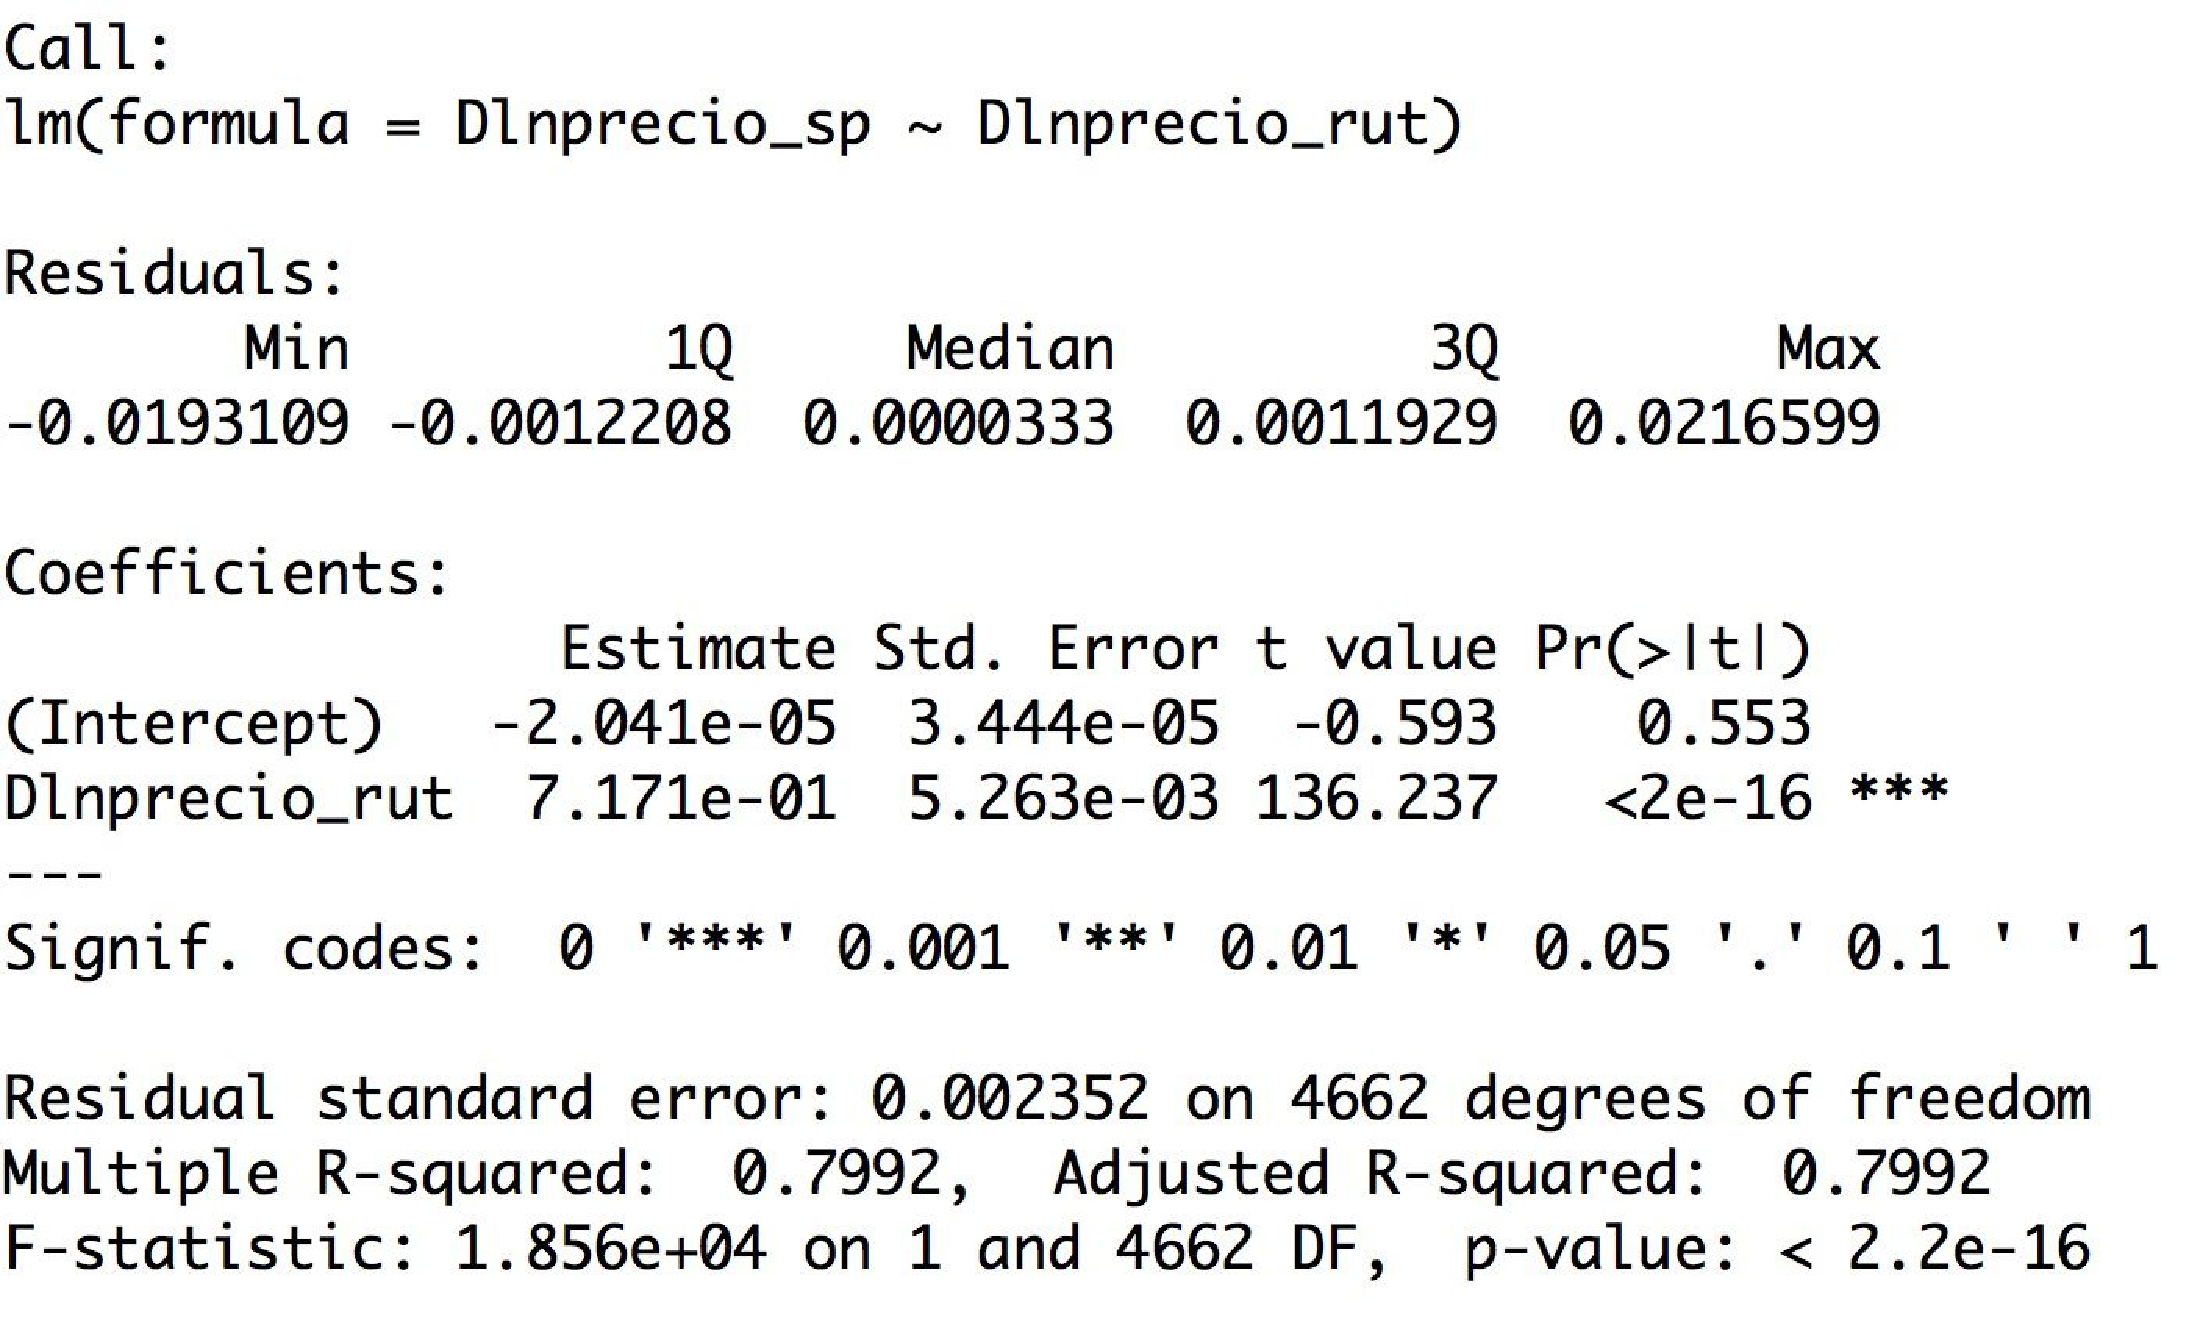
\includegraphics[width=\linewidth]{reg1.pdf}}
%	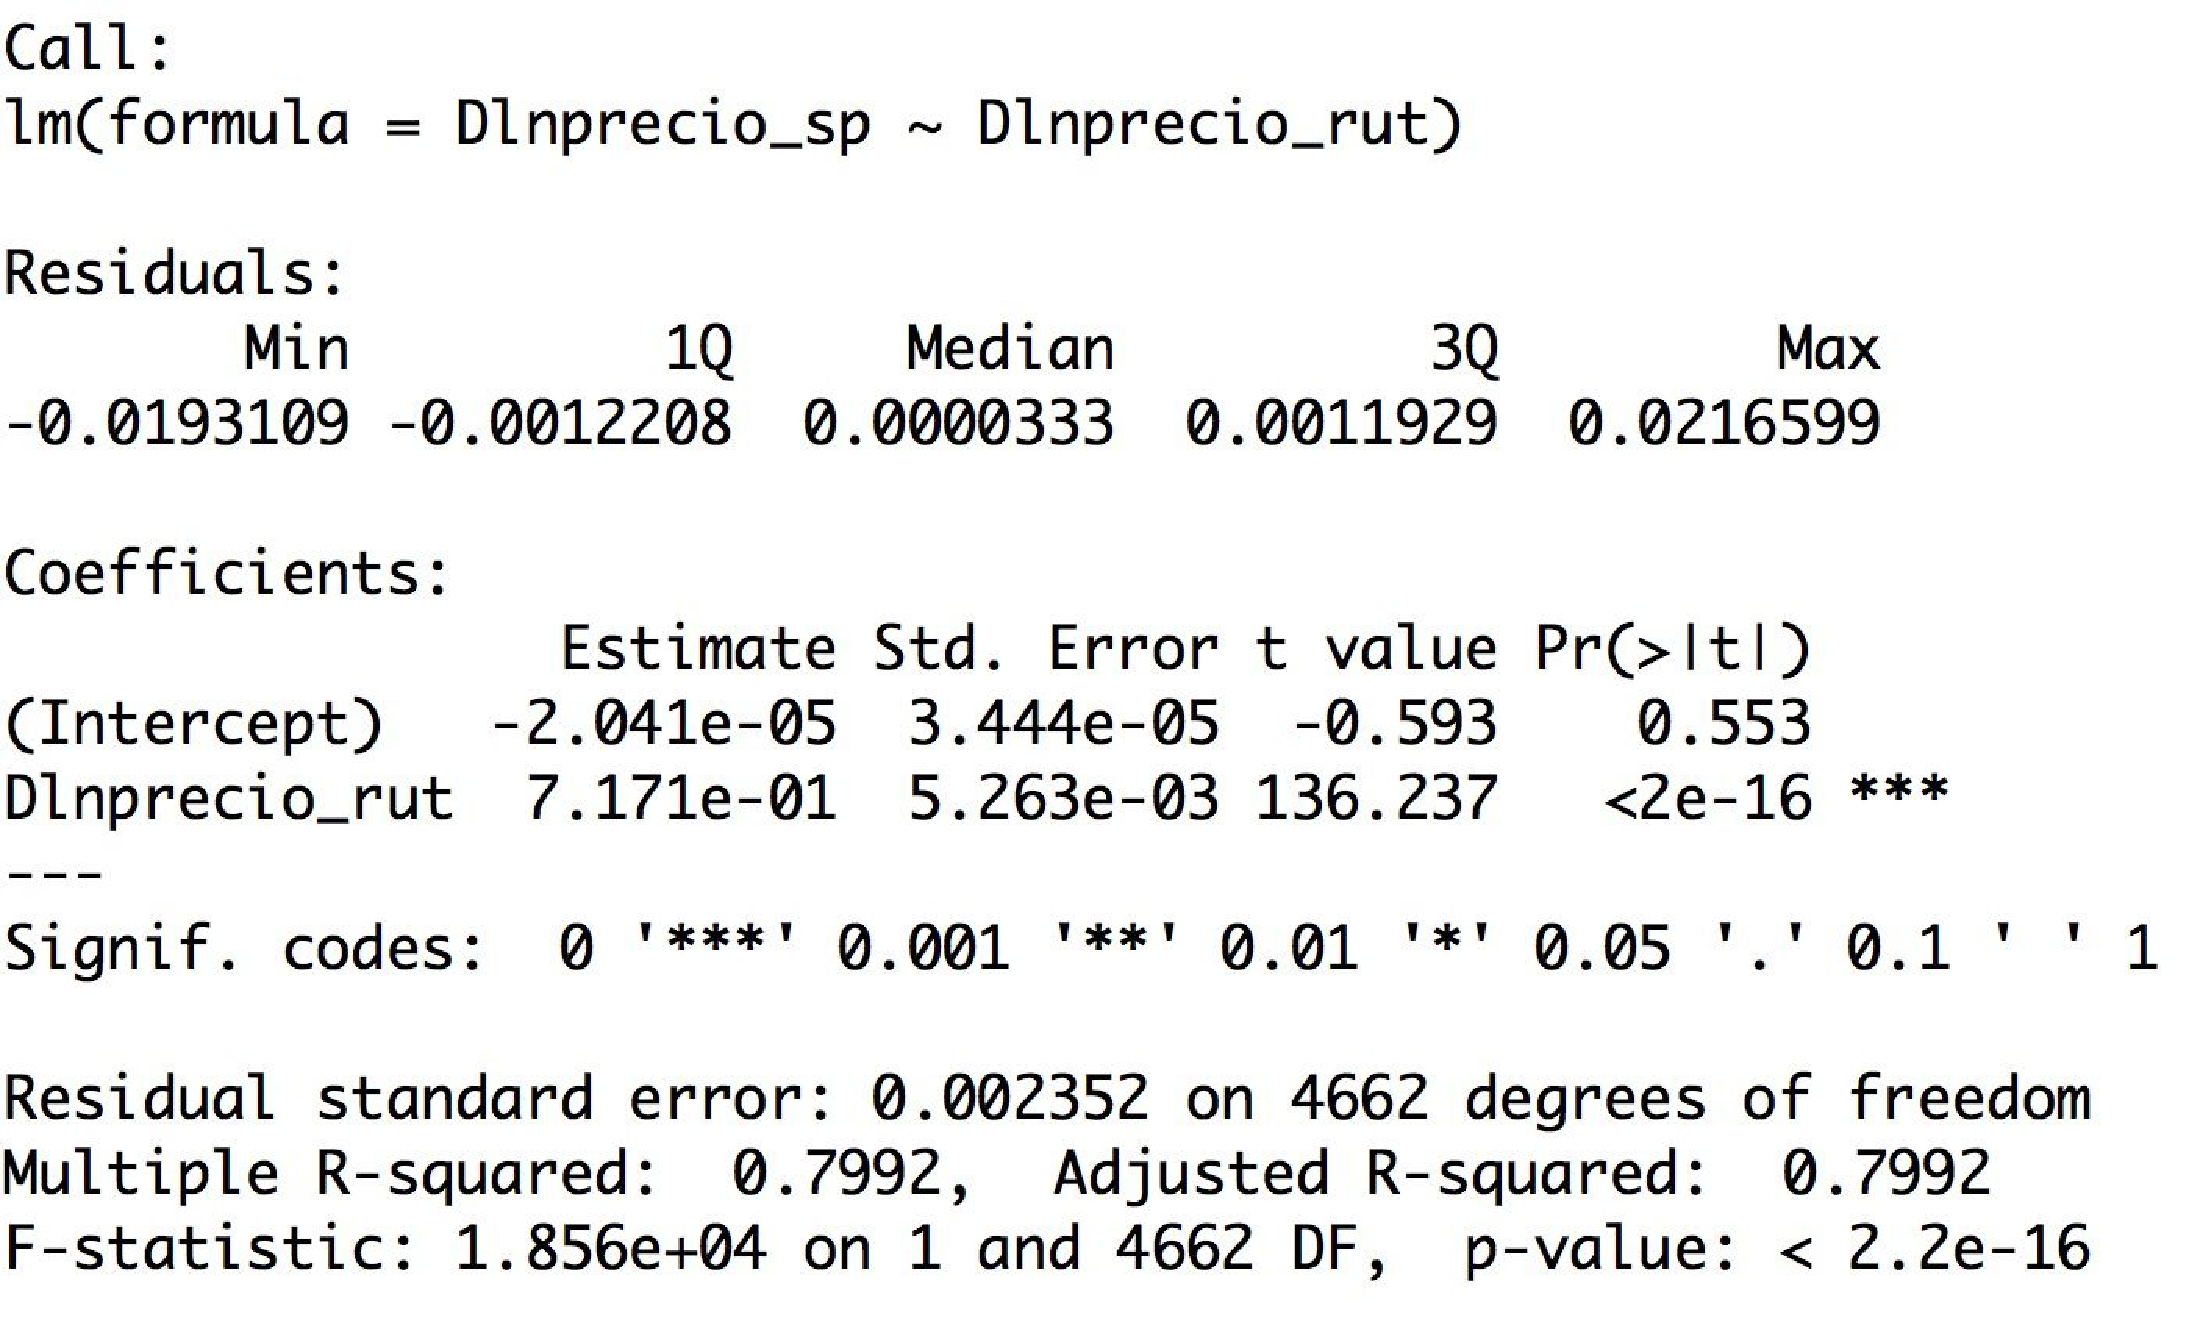
\includegraphics[scale=0.34]{reg1.pdf}
\end{figure}

%\end{frame}
%---------------------------------------------------------

%---------------------Slide 61 --------------------------
%\begin{frame}
%\frametitle{Ejemplo 3: Regresiones}
\lstset{caption = Código R para Regresiones,framexleftmargin=5mm, frame=shadowbox, rulesepcolor=\color{green}}
\begin{lstlisting}[title={‘Código R para Regresiones’},basicstyle=\ttfamily]{}
mydata1 <- read.csv("sp.csv", header=TRUE, 
					stringsAsFactors=FALSE)
precio_sp <- mydata1$"Adj.Close"; 
lnprecio_sp <- log10(precio_sp)
Dlnprecio_sp <- diff(lnprecio_sp ,1)
mydata2 <- read.csv("rut.csv", header= TRUE,
				stringsAsFactors = FALSE)
precio_rut <- mydata2$"Adj.Close" ; 
lnprecio_rut <- log10(precio_rut)
Dlnprecio_rut <- diff(lnprecio_rut ,1)
reg1 <- lm ( Dlnprecio_sp ~ Dlnprecio_rut)
summary(reg1)
\end{lstlisting}\label{ejemplo3Regresiones}
%
%\only<1|handout:1>{
%	\begin{exampleblock}{C\'odigo en R}
%		rm(list=ls())\\
%		mydata $<-$ read.csv (``/Users/marcelovillena/Desktop/sp.csv", header = TRUE, stringsAsFactors = FALSE)\\
%		$precio\_sp$ $<-$ mydata$\$$``Adj.Close" : $lnprecio\_sp$  $<-$ log10($precio\_sp$ ) ; $Dlnprecio\_sp$  $<-$ diff($lnprecio\_sp$ ,1)\\
%		mydata $<-$ read.csv (``/Users/marcelovillena/Desktop/rut.csv", header = TRUE, stringsAsFactors = FALSE)\\
%		$precio\_rut$ $<-$ mydata$\$$``rut" ; lnprecio\_rut  $<-$ log10($precio\_rut$ ) ; $Dlnprecio\_rut$  $<-$ diff($lnprecio\_rut$ ,1)\\
%		reg1 $<-$ lm ( $Dlnprecio\_sp$ $\string ~$ $Dlnprecio\_rut$)\\
%		summary(reg1)
%	\end{exampleblock}
%}
%\end{frame}
%---------------------Slide 62 --------------------------
%\begin{frame}
%\frametitle{Ejemplo 3: Regresioness}

\begin{figure}[H]
	\centering
	\textbf{Russell explicado por SP500}\par\medskip
	\fcolorbox{green}{blue}{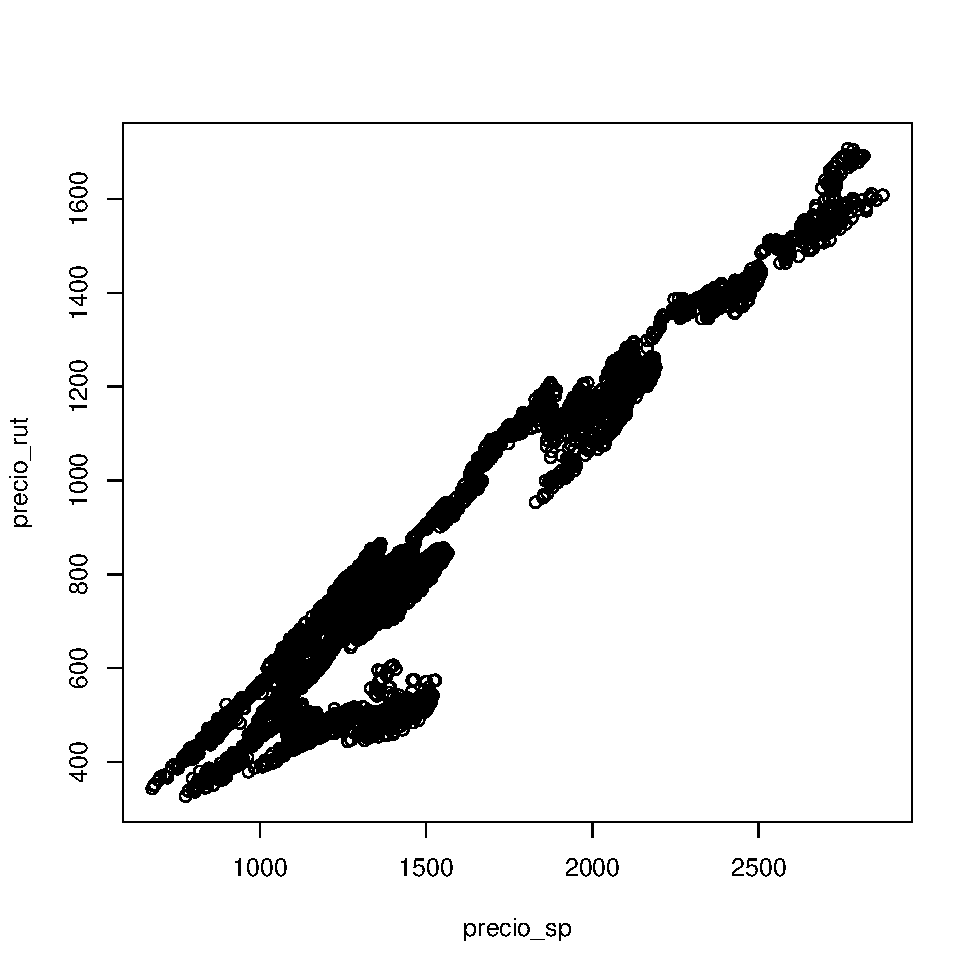
\includegraphics[width=\linewidth]{graph_precios.pdf}}
%	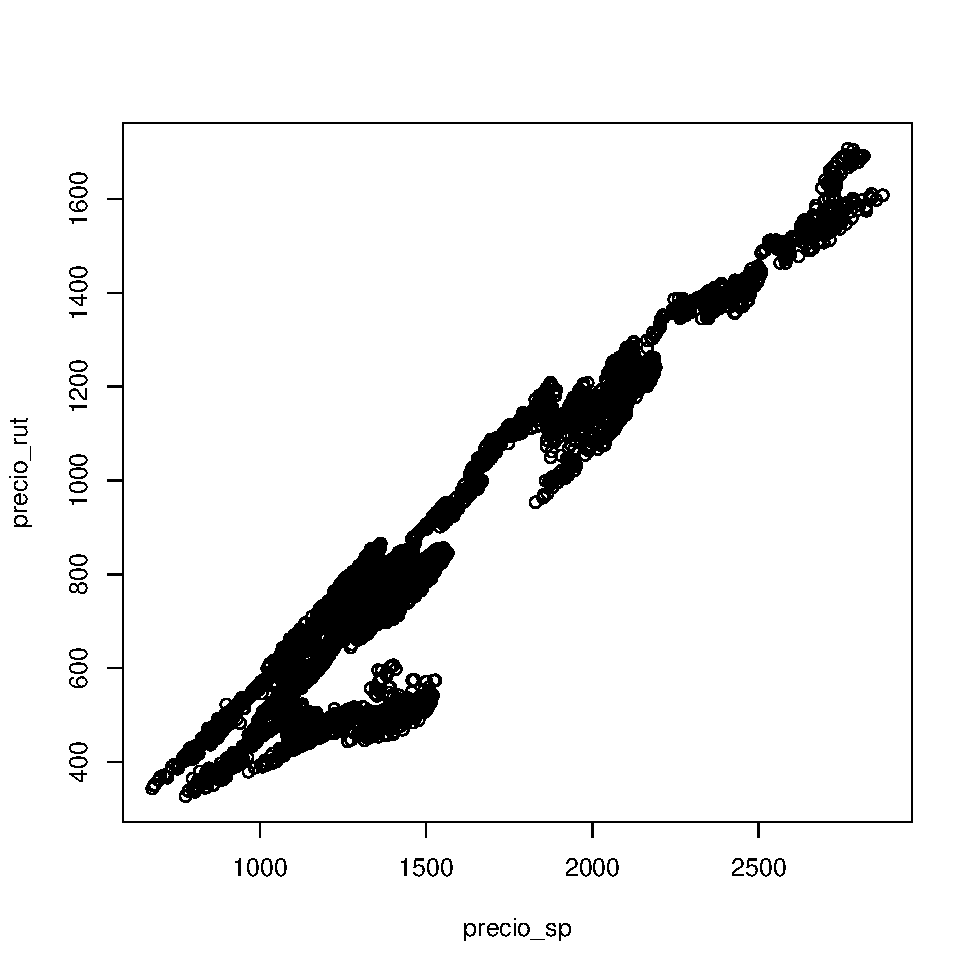
\includegraphics[scale=0.6]{graph_precios.pdf}
	\caption{Regresión de Russell 2000 en función del S\&P500}
\end{figure}

%\end{frame}

%---------------------------------------------------------	
%---------------------Slide 63 --------------------------
%\begin{frame}
%\frametitle{Ejemplo 3: Regresiones}

\pagebreak A partir del siguiente c\'odigo almacenamos los residuos y analizamos los supuestos que exige una buena regresi\'on.
\lstset{caption = Código R para Residuos,framexleftmargin=5mm, frame=shadowbox, rulesepcolor=\color{green}}
\begin{lstlisting}[title={‘Código R para Residuos de regresión’},basicstyle=\ttfamily]{}
residuos <- rstandard(reg1)
valores.ajustados <- fitted(reg1)
plot(valores.ajustados, residuos)
qqnorm(residuos)
qqline(residuos)
\end{lstlisting}\label{ejemplo3ResiduosRegresion}
%\only<1|handout:1>{
%	\begin{exampleblock}{C\'odigo en R}
%		residuos $<-$ rstandard(reg1)\\
%		valores.ajustados $<-$ fitted(reg1)\\
%		plot(valores.ajustados, residuos)\\
%		qqnorm(residuos)\\
%		qqline(residuos)\\
%	\end{exampleblock}
%}
%\end{frame}
%---------------------Slide 54 --------------------------
%\begin{frame}
%\frametitle{Ejemplo 3: Regresiones}



\begin{figure}[H]
	\centering
	\textbf{Homocedasticidad}\par\medskip
	\fcolorbox{green}{blue}{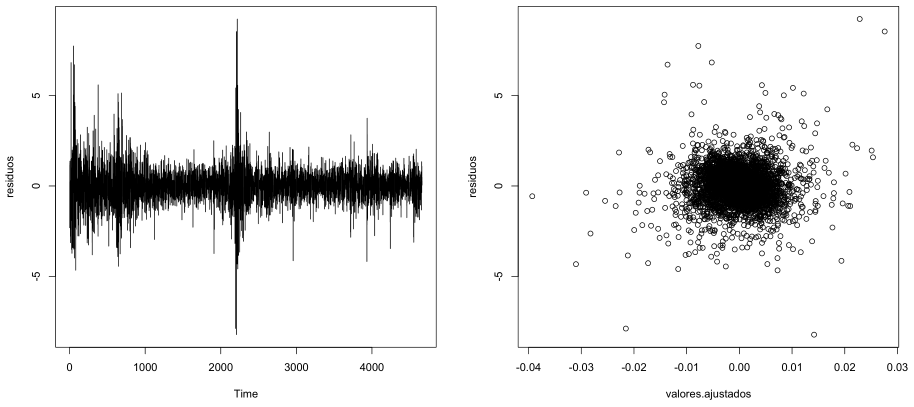
\includegraphics[width=\linewidth]{homocedasticidadD64.png}}
%	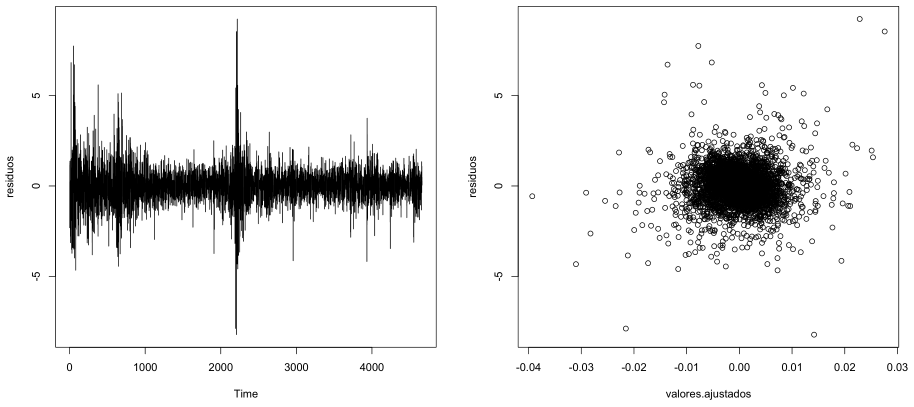
\includegraphics[scale=0.5]{homocedasticidadD64.png}

	\caption[Homocedasticidad]{Izquierda: Derecha}\label{fig11}
\end{figure}

%\end{frame}
%---------------------------------------------------------
%---------------------Slide 65 --------------------------
%\begin{frame}
%\frametitle{Ejemplo 3: Regresiones}



\begin{figure}[H]
	\centering
	\textbf{Normalidad de los residuos}\par\medskip
	\fcolorbox{green}{blue}{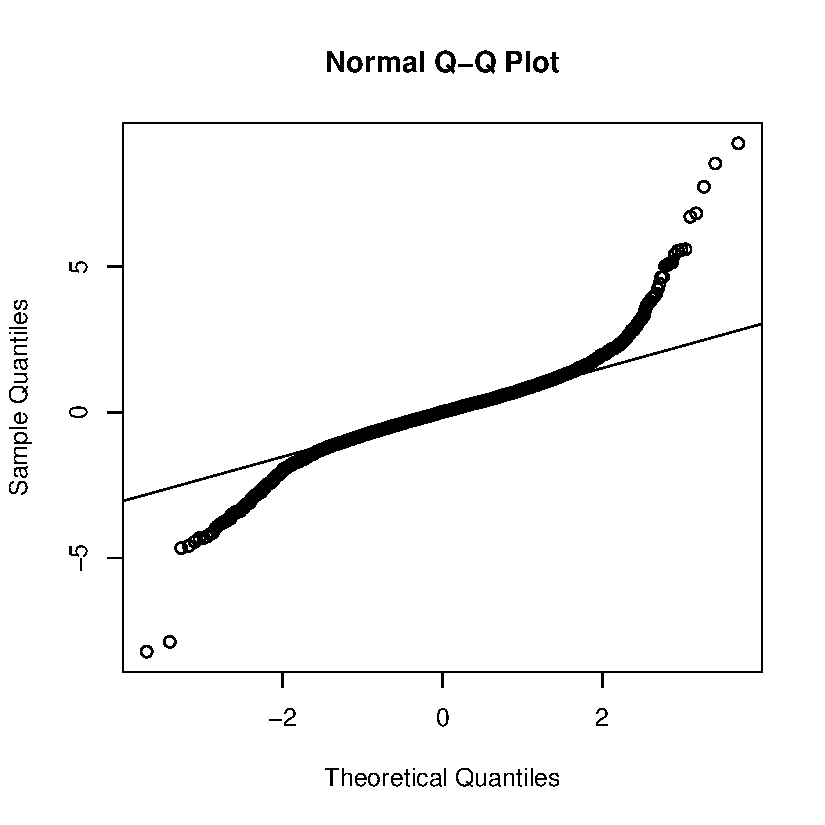
\includegraphics[width=\linewidth]{qqplot_reg1.pdf}}
	\caption{Grafico QQ-Plot de los residuos. La linea punteada indica el comportamiento de una distribución normal, mientras los puntos alejados de ella en los extremos dan cuenta de como se alejan los residuos del comportamiento normal.}
\end{figure}\label{fig12}

%\end{frame}
%\end{section}















%\section{Table}
%
%\begin{table}[htp]
%    \centering
%    \begin{tabular}{r|l|p{10cm}}
%        Right &  Left  &  Longlonglonglonglonglonglonglong longlonglonglonglonglonglonglonglonglonglonglonglong longlonglonglonglonglong \\
%        Right &  Left  &  Longlonglonglonglonglonglong
%        longlonglonglonglonglonglonglong
%        longlonglonglong
%        longlonglonglonglonglonglonglong 
%    \end{tabular}
%    \caption{This is a caption}
%    \label{tab:trans-sym}
%\end{table}
%
%\section{List}
%This is a List:
%\begin{itemize}
%    \item \textbf{Bullet 1}: Bullet 1 is bullet 1.
%    \item \textbf{Bullet 2}: Bullet 2 is bullet 2.
%\end{itemize}
%
%\section{Definition}
%\begin{definition}\label{def:def117}
%\textbf{DEFINITION NAME}: This is a definition.
%\end{definition} 
%
%% avoid bad break
%\vspace{5cm} 
%
%\section{Theorem}
%\begin{theo}[THEOREM NAME]{theo:theo1}
%This is a theorm. Below are equations.
%\begin{align}\label{eq:multi-equations}
%    \psi(\bvec{a}) &= A\cdot \bvec{a} + \bvec{t}.\\
%    R_x &=  \begin{bmatrix} 
%            0 & \cos(\theta) & -\sin(\theta)\\
%            0 & \sin(\theta) & \cos(\theta)\\
%            1 & 0 & 0
%         \end{bmatrix}, 
%    R_y =  \begin{bmatrix} 
%            \cos(\theta) & 0 & -\sin(\theta)\\
%            \sin(\theta) & 0 & \cos(\theta)\\
%            0 & 1 & 0
%         \end{bmatrix}, 
%    R_z =  \begin{bmatrix} 
%            \cos(\theta) & -\sin(\theta) & 0\\
%            \sin(\theta) & \cos(\theta) & 0 \\
%            0 & 0 & 1
%         \end{bmatrix} 
%\end{align}
%\end{theo}
%
%\begin{lem}[LEMMA NAME]{lem:leml}
%This is a lemma
%\end{lem}
%
%\begin{prf}[LEMMA NAME]{prf:leml}
%This is a proof.
%\end{prf}
%
%\section{Tikz Pictures}
%\begin{figure}[htp]
%    \centering
%        \begin{tikzpicture}[scale=0.6]
%            \draw[->] (0,-1)--(0,1.5)node[above] {$s$};
%            \draw[->] (-0.8,0.6) to[bend right] (0.8,0.6);
%            \draw[->] (0.9, 0.8)--(0.9, 1.2) node[right] {$\omega$};
%            \filldraw[dashed] (0,-0.2)--(0.9, -0.3) circle (1pt) node [right] {$q$};
%            \draw[->] (0.8, -0.9)--(1.2, -0.8) node[right] {$v$};
%        \end{tikzpicture}
%    \caption{This is a caption. }
%    \label{fig:rotation}
%\end{figure}

\curinstructor{Marcelo Villena Chamorro PhD.}